\documentclass[a4paper]{report}

%----------------------------------------------------------------------------------------
%	PRE-DOCUMENT PAGES
%----------------------------------------------------------------------------------------
%
%\makeglossaries
%
%\graphicspath{{img/}}
%\setmarginsrb{3 cm}{2.5 cm}{3 cm}{2.5 cm}{1 cm}{1.5 cm}{1 cm}{1.5 cm}
\newcommand\myworries[1]{\textcolor{red}{#1}}

%----------------------------------------------------------------------------------------
%	LATEX BUILD INFO
%----------------------------------------------------------------------------------------

%!TEX root = report.tex
\usepackage{color}
%\usepackage{enumitem}
\usepackage{datetime}
\usepackage{courier}
\usepackage{titlesec}
\usepackage{longtable}
% \usepackage{float}
\usepackage[hidelinks]{hyperref}
\usepackage{booktabs}
\usepackage[table,xcdraw,svgnames]{xcolor}
\usepackage{listings}
\usepackage{fancyhdr}

%\usepackage{listings}
%\usepackage[figure,table,lstlisting]{totalcount}
\usepackage{etoolbox}% http://ctan.org/pkg/etoolbox
\usepackage{graphicx}% http://ctan.org/pkg/graphicx
\usepackage{lipsum}

% add the command \conditionalLoT
% that only displays the list of tables,
% if any tables are defined
\makeatletter
\AtEndEnvironment{table}{\gdef\there@is@a@table{}} 
\AtEndDocument{\ifdefined\there@is@a@table\label{table:was:used:in:doc}\fi} 
\newcommand{\conditionalLoT}{\@ifundefined{r@table:was:used:in:doc}{}{
	\addcontentsline{toc}{section}{List of Tables}	
	\clearpage
	\listoftables
}}%

% same as above, but then with list of figures
\AtEndEnvironment{figure}{\gdef\there@is@a@figure{}} 
\AtEndDocument{\ifdefined\there@is@a@figure\label{figure:was:used:in:doc}\fi} 
\newcommand{\conditionalLoF}{\@ifundefined{r@figure:was:used:in:doc}{}{
	\clearpage
	\addcontentsline{toc}{section}{List of Figures}
	\listoffigures
}}%


\makeatother


%remove the blank page while using landscape:
\usepackage{afterpage}

\usepackage[]{floatpag}

\usepackage[hypcap,tableposition=top]{caption}
%\usepackage{natbib}
%\usepackage{url}
%\usepackage[utf8x]{inputenc}
%\usepackage{amsmath}
%\usepackage{graphicx}
%\usepackage{parskip}
%\usepackage{fancyhdr}
%\usepackage{vmargin}
%\usepackage{xcolor}
%\usepackage{nameref}
%
%\usepackage[hypcap]{caption}

%to reference multiple things at once:
%like \cref{fig:1, fig:2}
%\usepackage{cleveref}

%to frame text with a border
\usepackage{framed}

%to rotate images
\usepackage{rotating}
%usd to cite multiple things at once
% like \cite{citate1, citate2}
%\usepackage{cite}

%used to create lists without any spacing
\usepackage{adjustbox}

%to serperate the table style from the data
\usepackage{pgfplotstable}

%to make a compact itemize list in a table
%\usepackage{paralist}


% To make the table captions on top
% \let\newfloat\relax
\usepackage{floatrow}

% Accept é ë etc
\usepackage[utf8]{inputenc}
\usepackage[T1]{fontenc}
% Thanks, Laura Baakman

%Show todonotes:
%\usepackage{todonotes}
%Hide todonotes:
\usepackage[disable]{todonotes}

% For shoing euro currency
\usepackage[gen]{eurosym}

%%%%
\usepackage{selinput}
\usepackage[margin=2cm]{geometry}
\usepackage{enumitem,varwidth}
\usepackage{tikz}
\usetikzlibrary{shapes.geometric}
\usepackage{lmodern}
%%%%%%

% parskip puts a lot more white space in to the paper
% I (Guus) prefer it as it allows me te distinguish text
% way faster. However, it's preference, so we could 
% also remove it, if people feel that is needed
\usepackage{parskip}

\usepackage{pbox}
\usepackage[toc]{appendix}

% These packages are used for rotating table header
\usepackage{array}
\usepackage{graphicx}
\usepackage{booktabs}
\usepackage{pifont}

% To determine if a space is needed or not
\usepackage{xspace}
\usepackage{amsmath}

%\usepackage[nopostdot,nonumberlist,toc,acronym,nogroupskip,xindy]{glossaries}
\usepackage[nopostdot,nonumberlist,acronym,nogroupskip]{glossaries}
\setglossarystyle{altlist}

%\usepackage[toc]{glossaries}
%\usepackage[acronym]{glossaries}


%remove the blank page while using landscape:
\usepackage{afterpage}

% For landscape page
\usepackage{pdflscape}
%!TEX root = report.tex

\newcommand{\q}[1]{``#1''}

\newcommand{\code}[1]{\textbf{\texttt{\uppercase{#1}}}}
\newcommand{\codeu}[1]{\textbf{\code{#1}}}



\newcommand{\todonote}[1]{\textcolor{red}{#1}}
\newcommand{\attention}[1]{\textcolor{green}{#1}}
\newcommand{\HRule}{\rule{\linewidth}{0.5mm}}
\newcommand{\cellBox}[1]{\pbox{0.6\textwidth}{#1}}
%\newcommand\myworries[1]{\textcolor{red}{#1}}
\newcommand\myworries[1]{}

\newcommand{\ign}[1]{}

% Commands for rotating table header
\newcommand*\rot{\rotatebox{90}}
\newcommand*\OK{\ding{51}}

\newcommand{\compactCell}[1]{%
    \adjustbox{valign=t}{%
        \begin{minipage}{\linewidth}%
            #1%
        \end{minipage}%
    }%
}

\newcommand{\compactList}[2]{%
    %\begin{minipage}[t][][p]{\linewidth}%
    %\begin{minipage}{\linewidth}%
    \adjustbox{valign=t}{%
        \begin{minipage}{\linewidth}
            \begin{#1}[%
                nosep,
                nolistsep,
                topsep=1pt,
                partopsep=0pt,
                parsep=0pt,
                %itemsep=0pt,
                itemindent=0pt,
                %labelsep=*,
                %align=margin,
                align=left,
                %leftmargin=\linewidth,
                leftmargin=*,
                labelwidth=*,
                after=\strut,
                ]#2\end{#1}%
        \end{minipage}%
    }%\end{adjustbox}
}%

\newcommand{\allotOfText}{%
    LaTeX styled as LATEX, and a shortening of Lamport TeX is a word processor and a document markup language. It is distinguished from typical word processors such as Microsoft Word and Apple Pages in that the writer uses plain text as opposed to formatted text, relying on markup tagging conventions to define the general structure of a document (such as article, book, and letter), to stylise text throughout a document (such as bold and italic), and to add citations and cross-referencing. A TeX distribution such as TeXlive or MikTeX is used to produce an output file (such as PDF or DVI) suitable for printing or digital distribution.
}
%
%\newcolumntype{R}[2]{%
%    >{\adjustbox{angle=#1,lap=\width-(#2)}\bgroup}%
%    l%
%    <{\egroup}%
%}
%\newcommand*\rotmc{\multicolumn{1}{R{90}{1em}}}% no optional argument here, please!
%

%\newcolumntype{R}[2]{%
%    >{\adjustbox{angle=#1,lap=\width-(#2)}\bgroup}%
%    l%
%    <{\egroup}%
%}
%\newcommand*\rot{\multicolumn{1}{R{90}{1em}}}% no optional argument here, please!


%command to decrease the size it takes to write
%L{0.5\textwidth}. This will now be:
%L{\tw{0.5}}. A small difference, but it adds up
\newcommand{\tw}[1]{#1\textwidth}

\newcommand\crule[3][black]{\textcolor{#1}{\rule{#2}{#3}}}


\newcommand{\getNr}[1]{%
    \getNext{#1}
    \arabic{#1}
}

\makeatletter

%manually lable something
%like \manuallabel{fr:01}{The first }
% \ref{fr:01} will then hold "The first req"
\newcommand{\manuallabel}[2]{\def\@currentlabel{#2}\label{#1}}

\newcommand{\getNext}[1]{%
    %check if counter with that name excists
    \@ifundefined{c@#1}
    {% the counter doesn't exist
        \newcounter{#1}\setcounter{#1}{1}%
    }
    {% the counter exists
        \stepcounter{#1}%
    }%
}
\newcommand{\nextNrRef}[1]{%
\getNext{#1}
\manuallabel{#1:\arabic{#1}}
{\uppercase{#1}-\arabic{#1}}
\arabic{#1}
}


\newcommand{\req}[1]{%
    \uppercase{#1}-\nextNrRef{#1}
}

\newcommand{\frReqRowNoRule}[3]{%
    \phantomsection
    \getNext{FR}
    \manuallabel{fr:#1}{FR-\arabic{FR}} 	
    FR-\arabic{FR} &
    \ifcase\pdfstrcmp{#2}{Must}%
    \textbf{#2}
    \else
    #2
    \fi
    &
    #3
    \\

}

\newcommand{\frReqRow}[3]{%
    \midrule
    \frReqRowNoRule{#1}{#2}{#3}
}	

\newcommand{\newshortlabel}[2]{\phantomsection\getNext{#1}\manuallabel{#1:#2}{\uppercase{#1}-\arabic{#1}}\uppercase{#1}-\arabic{#1}}

\newcommand{\nsl}[2]{\newshortlabel{#1}{#2}}


\newcommand{\hlReqRow}[4]{%
    \midrule
    \\
    \phantomsection
    \req{HL} &
    \ifcase\pdfstrcmp{#2}{Must}%
    \textbf{#2}
    \else
    #2
    \fi
    & \textbf{#3} \\
    & & #4
    \\
    \\
}

\newcommand{\reqRow}[4]{%
    \midrule
    \phantomsection
    \req{#1}
    \manuallabel{#1:#2}{\uppercase{#1}-\arabic{#1}} &
    \ifcase\pdfstrcmp{#3}{Must}%
    \textbf{#3}
    \else
    #3
    \fi
    &
    #4
    \\
}		

\newcommand{\risk}[7]{%
    \begin{table}[H]
        \begin{tabular}{L{0.3\textwidth} L{0.7\textwidth}}\toprule\phantomsection\getNext{#1-RISK}\manuallabel{#7}{#1-RISK\arabic{#1-RISK}}\textbf{#1-RISK\arabic{#1-RISK}} & \textbf{#2} \\*
            \midrule
            \textbf{Probability of occurrence} & #3 \\*
            \midrule
            \textbf{Consequences}              & #4 \\*
            \midrule
            \textbf{Prevention}                & #5 \\*
            \midrule
            \textbf{Reaction}                  & #6 \\*
            \bottomrule
        \end{tabular}
        \caption{#1-RISK\arabic{#1-RISK} -- #2}
    \end{table}
    \vspace{0.5cm}
}

\newcommand{\pattern}[1]{%
	{\fontfamily{qcr}\selectfont\uppercase{#1}}}

\makeatother


%\makeatletter
%\newcommand{\req}[1]{%
%	\newcommand{\curCountVal}{\arabic{\getNr{#1}}}
%	\label{\curCountVal}
%}
%\makeatother

%	\label{#1:\arabic{#1}}
%	\arabic{#1}

% Glossary macros
\newcommand{\qos}{Quality of Service\xspace}

%!TEX root = report.tex
\setlist[itemize]{topsep=0pt,itemsep=-1ex,partopsep=1ex,parsep=1ex,after=\vspace{\baselineskip}}
\setlist[enumerate]{topsep=0pt,itemsep=-1ex,partopsep=1ex,parsep=1ex,after=\vspace{\baselineskip}}
\titleformat{\chapter}{\normalfont\LARGE\bfseries}{\thechapter}{1em}{}
\titlespacing*{\chapter}{0pt}{3.5ex plus 1ex minus 0.2ex}{2.3ex plus 0.2ex}
\newdateformat{mydate}{\twodigit{\THEDAY}{ }\shortmonthname[\THEMONTH], \THEYEAR}
\restylefloat{table}
% The example architecture document numbers subsubsections (3.2.1)
% And it those subsubsections are also included in the table of content
% The following commands make sure that this numbering/listing happens as in the example.

%\begingroup
\setlength{\LTleft}{-20cm plus -1fill}
\setlength{\LTright}{\LTleft}
%\endgroup

%To number subsubsections:
\setcounter{secnumdepth}{3}

%To include subsubsections in the table of contents:
\setcounter{tocdepth}{3}

%Nice custom column type
\newcolumntype{L}[1]{>{\raggedright\let\newline\\\arraybackslash}p{#1}}

\pgfplotstableset{%
    string type,
    col sep=&,
    row sep=\\,
    begin table={%
        %\begin{minipage}{\linewidth}
        \begin{longtable}
        },
        end table={%
        \end{longtable}
        %\end{minipage}
    },
    %every head row/.append style={after row=\endhead},
    %rows/0/.append style={after row=\endhead},
    %every table/.append style={outfile={#1.out}}
    %generate an outfile name for every table
}

\makeatletter

% \def\getcell#1#2#3{
% \pgfplotstablegetelem{#1}{#2}\of{#3}\pgfplotsretval%

\pgfplotstableset{%
    string type,
    col sep=&,
    row sep=\\,
    begin table={%
        %\begin{minipage}{\linewidth}
        \begin{longtable}
        },
        end table={%
        \end{longtable}
        %\end{minipage}
    },
    bold/.append style={
        postproc cell content/.append code={%
            \pgfkeysalso{@cell content=\textbf{##1}}%
        },
    },
    highlight last row/.style={
        postproc cell content/.append code={
            \count0=\pgfplotstablerow
            \advance\count0 by1
            \ifnum\count0=\pgfplotstablerows
            \pgfkeysalso{@cell content=\textbf{##1}}%
            \fi
        },
    },
    %    bold header/.append style={
    %		column type={>{\fontseries{bx}\selectfont}l},
    %		postproc cell content/.append code={
    %			\pgfkeysalso{@cell content={\fontseries{\seriesdefault}\selectfont}{}}}
    %    },
    bold header/.append style={
        column type={>{\fontseries{bx}\selectfont\centering\arraybackslash}c},
        postproc cell content/.append style={
            /pgfplots/table/@cell content/.add={\fontseries{\seriesdefault}\selectfont}{}}
    },		
    UCTable/.append style={
        %		begin table={%
        %			\begin{minipage}{\linewidth}
        %			\begin{longtable}[c]
        %		},
        %		end table={%
        %			\end{longtable}
        %			\end{minipage}
        %		},
        every head row/.style={
            output empty row,
            before row={},
            after row={},
        },
        every last row/.style={%
            after row=\bottomrule,
        },
        columns/value/.style={
            bold,
            column type=L{\tw{0.2}},
        },
        columns/description/.style={
            column type=L{\tw{0.6}},
        },
        before row=\midrule,
    },
    KeyValue/.append style={
        every head row/.style={
            output empty row,
            before row={},
            after row={},			
        },
        every last row/.style={%
            after row=\bottomrule,
        },
        columns/key/.style={
            column type=L{\tw{0.3}},
        },
        columns/value/.style={
            column type=L{\tw{0.6}},
        },
        before row=\midrule,
    },
    Costs/.append style={
        KeyValue,
        display columns/0/.style={
            column name={\textbf{Description}},column type = {l},string type
        },
        display columns/1/.style={
            column name={\textbf{Cost}},fixed,column type = {r}
        },		
    }		
}


\title{Smart Flood Monitoring}		

\author{
		\texttt{Putra, Guntur}\\
		\texttt{Fakambi, Aur\'{e}lie}\\
		\texttt{Schaefers, Joris}\\
		\texttt{Menninga, Wouter}\\
}

\date{\today}											% Date

\makeatletter
\let\thetitle\@title
\let\theauthor\@author
\let\thedate\@date
\makeatother


%\pagestyle{fancy}
%\fancyhf{}
%\cfoot{\thepage}

\floatpagestyle{empty}
%\thispagestyle{}
%\thisfloatpagestyle{empty}

\renewcommand{\sectionmark}[1]{\markright{\iffloatpage{}{\thesection.\ #1}}}
\fancyhf{} % delete current setting for header and footer
\fancyhead[LE,RO]{\iffloatpage{}{\textbf{Page \thepage\ of \pageref{LastPage}}}}
\fancyhead[LO]{\iffloatpage{}{\textbf\rightmark}}
\fancyhead[RE]{\iffloatpage{}{\textbf\leftmark}}
\fancyfoot[C]{\iffloatpage{\textbf{Page \thepage\ of \pageref{LastPage}}}{}}
\renewcommand{\headrulewidth}{\iffloatpage{0pt}{0.5pt}}
\renewcommand{\footrulewidth}{0pt}
%\renewcommand{\headsep}{10pt}


%\addtolength{\headheight}{\baselineskip} % make space for the rule
%\fancypagestyle{plain}{%
%	\fancyhead{} % get rid of headers on plain pages
%	\renewcommand{\headrulewidth}{0pt} % and the line
%}

\begin{document}

%----------------------------------------------------------------------------------------
%	VARIABLES
%----------------------------------------------------------------------------------------

\newcommand{\VersionNumber}{1.0}
\newcommand{\CompanyName}{RugSAG3\xspace}
\newcommand{\ProjectName}{Smart Monitoring\xspace}
\newglossaryentry{SFM}{name=SFM, description={Smart Flood Monitoring}}

\bibliographystyle{plain}

%!TEX root = report.tex
%----------------------------------------------------------------------------------------
%	TITLE PAGE
%----------------------------------------------------------------------------------------

%%%%%%%%%%%%%%%%%%%%%%%%%%%%%%%%%%%%%%%%%%%%%%%%%%%%%%%%%%%%%%%%

\begin{titlepage}
	\centering
    
    \vspace*{0.5 cm}
    
\includegraphics[scale = 0.25]{images/rug.png}\\[1.0 cm]	% University Logo
    \textsc{\LARGE University of Groningen}\\[0.3cm]
	\textsc{\large {Software Patterns}}\\
	\textsc{\large {Team 2}} \\[1.5 cm]
	\rule{\linewidth}{0.2 mm} \\[0.1 cm]
	{ \huge \bfseries \thetitle}\\
	
	\rule{\linewidth}{0.2 mm} \\[1.0 cm]

	
\includegraphics[scale = 0.5]{images/docker.png}\\[1.0 cm]	% Docker Logo
	
	\textbf{\large\emph\textbf{Authors:}}\\
	\theauthor
		
	~\\[0.8cm]	
	{\large \thedate}\\[0.25cm]
		Version \VersionNumber \\
		\renewcommand{\headrulewidth}{0pt}
	\vfill

%	\fancypagestyle{empty}{%
%		\fancyhf{}% Clear header/footer
%		\renewcommand{\headrulewidth}{0pt}
%%		\fancyfoot[C]{
%%			Version: \VersionNumber \\
%%			\mydate\today
%%		}
%	}
%	\iffloatpage{}{fancy}	
	
\end{titlepage}
\renewcommand{\headrulewidth}{0pt}
% Change the page numbering to roman ("i", "ii", etc) for the first few pages
\setcounter{page}{1}
\pagenumbering{roman}

\addcontentsline{toc}{section}{Revisions}
%!TEX root = ../report.tex
\section*{Authors}

\begin{tabular}{L{\tw{0.45}} L{\tw{0.45}}}
	\textbf{Name}        & \textbf{E-Mail}               \\ \toprule
	Putra, Guntur        & G.D.Putra@student.rug.nl      \\
	Fakambi, Aur\'{e}lie & A.Fakambi@student.rug.nl      \\
	Schaefers, Joris     & J.Schaefers@student.rug.nl    \\
	Menninga, Wouter     & W.G.Menninga@student.rug.nl   \\ 
\end{tabular}

\section*{Revision History}
\begin{longtable}{L{\tw{0.1}} L{\tw{0.2}} L{\tw{0.1}} L{\tw{0.5}}}
	\textbf{Version} & \textbf{Author}       & \textbf{Date} & \textbf{Description}                                                                                                                                                                                                       \\ \endhead	\toprule
				%date:dd-mm-yy
				0.1 & Schaefers & 11-12-15 & \\
					& Putra		& 13-12-15 & First draft of introduction chapter. \\
					& Fakambi   & 11-12-15 & \\
					& Menninga  & 11-12-15 & \\
					& Menninga  & 11-12-15 & \\
				\midrule
%			
%				0.2 & Schaefers & 11-12-15 & \\
%					& Putra		& 11-12-15 & \\
%					& Fakambi   & 11-12-15 & \\
%					& Menninga  & 11-12-15 & \\
%					& Menninga  & 11-12-15 & \\
%				\midrule
\end{longtable}

\addcontentsline{toc}{section}{Table of Contents}
\tableofcontents

\clearpage

\addcontentsline{toc}{section}{List of Figures}
\listoffigures

\clearpage

\addcontentsline{toc}{section}{List of Tables}
\listoftables

% \clearpage

\addcontentsline{toc}{section}{Glossary}
\glsaddall
\printglossaries
\newpage

\thispagestyle{empty}

% Change the page numbering back to the normal 1,2,3 form starting at 1
\setcounter{page}{1}
\pagenumbering{arabic}

%----------------------------------------------------------------------------------------
%	START OF DOCCUMENT CONTENT
%----------------------------------------------------------------------------------------

%!TEX root = ../report.tex
\clearpage
\chapter{Introduction}
\label{ch:introduction}
This document presents architecture recovery of Docker\footnote{\url{https://www.docker.com/}} by identifying software patterns and performing an evaluation of the architecture based on the identified patterns. This document is part of the Software Pattern assignment at the University of Groningen.

Docker is an open-source project that automates the deployment of applications inside software containers, by providing an additional layer of abstraction and automation of operating-system-level virtualization on Linux \cite{dockerdef}.


This project utilizes the IDAPO\footnote{Identifying Architectural Patterns in Open Source Software} process to recover the architecture \cite{idapo}. The PBAR\footnote{Pattern-Based Architecture Reviews} approach is used to perform the evaluation \cite{pbar}.
% explain a bit more

% Make sure this part is there, in the final document
% ===================================================
% The IDAPO process consists of twelve steps. Step 1 corresponds to Sections 2 and 3, in which the type and domain of Apache is identified. Section 4 is related to Steps 2 to 5 where used technologies and candidate patterns are examined.

% Steps 6 to 12 is an iterative process, which results in the documentation of used patterns. The results are document in Section 5. During these steps, documentation, source code and the components and connectors have been studied. Furthermore, the identification and validation of patterns and variants has been realized.

% Along with IDAPO, the PBAR process determines the high-level process of pattern-based recovery and the evaluation of the architecture. The findings of this evaluation are documented in Section 6. An overview of the process mapping can be found in Appendix A2.

The rest of the document is explained as follows. Chapter \ref{ch:context} gives brief explanation with regard to Docker. Chapter \ref{ch:stakeholders} elaborates on the stakeholders involved in the Docker project and its corresponding key-drivers. Patterns discovered in the Docker project are documented in chapter \ref{ch:patterns}. Evaluation is presented in chapter \ref{ch:evaluation}. Chapter \ref{ch:recommendations} gives several recommendation for the Docker project. Lastly, a conclusion is drawn in chapter \ref{ch:conclusion}.

% !TEX root = ../report.tex
\chapter{System Context}
\label{ch:context}

In this chapter an global information about the Docker project is presented. This includes a general overview of the working of docker and the history of the docker project.

\section{Overview}
%TODO joris: Add citation for:
% 	main goal
%	dotCload
% 	first release

Docker is an open-source project, created by Solomon Hykes, written in the \q{Go} programming language \cite{golang}. The goal of docker is making the deployment and distribution of applications easier. Docker started as an internal project within dotCloud, a platform-as-a-service company with four main developers. The first open-source version of Docker was released in March 2013.\\

Docker automates the deployment of applications inside so-called \q{containers} by making use of operating-system-level virtualization.
They state that ``Docker provides an integrated technology suite that enables development and IT operations teams to build, ship, and run distributed applications anywhere''\cite{whatisdocker}.\\

%borrowed from bsc thesis
Operating-system-level virtualization is a virtualization method where the kernel of an operating system allows the isolation of multiple instances of the user space of the operating system. Leveraging this type of virtualization over full virtualization (i.e. hardware emulation) offers a significant performance increase, because there is no need for emulation of the hardware.\cite{VirtualizationTechnologies}

\begin{figure}[b!]
\centering
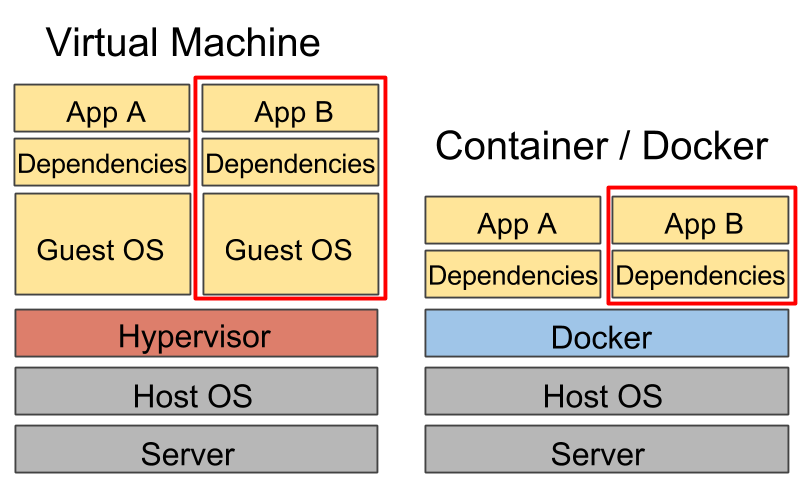
\includegraphics[scale=0.40,keepaspectratio=true]{./2-context/vmvsdocker}

\captionsource{Virtual machines compared to containers}{\cite{benchmarker}}
\label{fig:vmvsdocker}
\end{figure}

Figure \ref{fig:vmvsdocker} illustrates the difference between virtualization using hardware emulation and operating-system-level virtualization. As opposed to a virtual machine, a container does not have a guest operating system. Additionally, it does not need a hypervisor for emulating virtual hardware and trapping privileged instructions. This saves a lot of performance overhead. \\

One tool that makes use of operating-system-level virtualization is Docker. Docker can be used to package applications and dependencies in a `container'. Running this container using Docker will run it within a separate user space using operating-system-level virtualization. \\
Docker containers are instances of running Docker images. The process of creating a Docker image is relatively uncomplicated. It involves the creation of a so-called \q{Dockerfile}, which is a type of Makefile, containing instructions that are to be executed to install the application and dependencies (using the \codeu{run} instruction), and copy relevant data into the container (using \codeu{add}). Every Dockerfile extends another image (using the \codeu{from} instruction), which is either a previously created image or a base image (often containing the files of a specific operating system).

Docker images use a layered file system. Every command executed during the build-proces, creates a new layer where all modifications to the file system are stored.
Docker supports exporting images to tar-archive that are usable by similar versions of Docker.
%end of borrowed from bsc thesis



\section{Community}

% Always quote and reference https://www.docker.com/docker-community

Docker has an active community and the managers encourage developers around the world to contribute. \cite{dockeroswrittenfor}

There are several ways to get in contact with the community of Docker:
\begin{description}

\item [IRC] Here, the most knowledgeable Docker users reside. At the \verb|#docker| and \verb|#docker-dev| groups on \verb|irc.freenode.net|.

\item [Google Groups] The developers are active in the \verb|docker-dev| Google group.

\item [Stack Overflow] Questions about Docker itself can be asked on the Stack Overflow. 

\end{description}

The main organizations that contribute to Docker are:
\begin{itemize}
    \item Docker team
    \item Red Hat
    \item IBM
    \item Google 
    \item Cisco Systems
    \item Amadeus IT Group
\end{itemize}




% !TEX root = ../report.tex

\clearpage
\chapter{Stakeholders and Concerns}
\label{ch:stakeholders}
This section defines all stakeholders of the Docker system and describes the concerns of these stakeholders. A stakeholder is a person, group of persons, or organization that are involved in our system. This section uses the quality attributes as described in ISO-25010\cite{iso25010}.
% QA's from ISO-25010: https://nl.wikipedia.org/wiki/ISO_25010

% !TEX root = ../report.tex

\section{Stakeholders}
\label{sec:stakeholders}
This section presents the stakeholders and their concerns. We list the main concern in bold and, where applicable, the specific concern in parentheses.

%\item [Product owner] is the owner of the system. This stakeholder funds the project.  This affects the quality attributes usability and availability.
\subsection*{Software Developers}
The developers are those that use Docker to create their software systems. Docker is used by developers to deploy software and create architectures consisting of multiple containers. Developers using Docker for their system, expect it to work according to the documentation and have a good usability.
%TODO source

For Docker, we identified the following stakeholders:
\begin{itemize}
\item Software developers
\item Software Maintainers
\item Cloud providers
\item The open container initiative
\item Docker developers
\item Plugin developers
\end{itemize}

\textbf{Concerns}
\begin{description}[labelwidth=6cm,labelindent=30pt,style=multiline,leftmargin=5.5cm,font=\normalfont\itshape]

% Usuability
%		- Appropriateness recognizability. Degree to which users can recognize whether a product or system is appropriate for their needs.
%		- Learnability. degree to which a product or system can be used by specified users to achieve specified goals of learning to use the product or system with effectiveness, efficiency, freedom from risk and satisfaction in a specified context of use.
%		- Operability. Degree to which a product or system has attributes that make it easy to operate and control.
%User error protection. Degree to which a system protects users against making errors.
%		- User interface aesthetics. Degree to which a user interface enables pleasing and satisfying interaction for the user.
%		- Accessibility. Degree to which a product or system can be used by people with the widest range of characteristics and capabilities to achieve a specified goal in a specified context of use.

%Reliability
%		- Maturity. Degree to which a system, product or component meets needs for reliability under normal operation.
%		- Availability. Degree to which a system, product or component is operational and accessible when required for use.
%		- Fault tolerance. Degree to which a system, product or component operates as intended despite the presence of hardware or software faults.
%		- Recoverability. Degree to which, in the event of an interruption or a failure, a product or system can recover the data directly affected and re-establish the desired state of the system.

%Portability
%Adaptability. Degree to which a product or system can effectively and efficiently be adapted for different or evolving hardware, software or other operational or usage environments.
%Installability. Degree of effectiveness and efficiency with which a product or system can be successfully installed and/or uninstalled in a specified environment.
%Replaceability. Degree to which a product can replace another specified software product for the same purpose in the same environment.

\item[\textbf{Usability}] Since the software developers are using Docker, they want it to have good usability. This means it is easy to learn how to use Docker and it is not hard to work with. In fact, this is one of the main benefits of Docker, since it makes it easier to containerize applications, which could be done before, but was very difficult to do in practice.


\item[\textbf{Functional Suitability} (Functional correctness)] Software developers care about the functional correctness, since bugs in the Docker software make the development of their software more difficult. 

\end{description}

\subsection*{Software Maintainers}
Software maintainers are responsible for deploying the software and keeping the software product running. Docker is often used for software deployment (especially to the cloud). %TODO source
The software maintainers expect Docker to be reliable, portable, efficient and secure.

\textbf{Concerns}
\begin{description}[labelwidth=6cm,labelindent=30pt,style=multiline,leftmargin=5.5cm,font=\normalfont\itshape]

%[labelindent=25pt,style=multiline,leftmargin=4.0cm,font=\normalfont\itshape]

\item[\textbf{Reliability}] Software maintainers are responsible for keeping the software working while it is deployed. They will only use Docker if it is reliable. It has to be tolerant against failing containers.

\item[\textbf{Portability}] The software maintainers want to be able to run Docker and its containers on a variety of different environments.

\item[\textbf{Performance efficiency}] The software maintainers want Docker to have a good performance. They want the resources of their servers to be used as efficiently as possible and therefore want Docker to have almost no overhead, like Virtual Machines often do have.


\item[\textbf{Security}] Software maintainers want Docker to be secure, so they can run their applications inside the containers without Docker negatively affecting the security of their application.


\end{description}



\subsection*{Cloud providers}
There are numerous cloud providers offering services which are based on Docker\footnote{\url{https://www.docker.com/partners\#/service}}. These cloud providers offer Container-based cloud computing, sometimes referred to as CaaS (Containers-as-a-Service).


\textbf{Concerns}
\begin{description}[labelindent=25pt,style=multiline,leftmargin=4.0cm,font=\normalfont\itshape]

\item[\textbf{Portability} (Installability)] The cloud providers want to integrate Docker into their cloud computing architecture.\\ 

\item[\textbf{Compatibility} (Co-Existence)] Docker has to share the environment with the existing architecture of the cloud providers.

\item[\textbf{Reliability}] The customers using the cloud providers' services expect a high reliability. If cloud providers are to implement Docker in their architectures, they need Docker to have good reliability.

\item[\textbf{Security}] Cloud providers want to offer a secure cloud computing environment to their customers.
\end{description}



\subsection*{The Open Container Initiative}

The Open Container Initiative\footnote{\url{https://www.opencontainers.org/}} was formed with the purpose of creating an open industry standard for container formats and runtime in June 2015.

They are interested in creating a formal, open, industry specification around container formats and runtime. This specification should be independent of particular clients/orchestration stacks, commercial vendors or projects and should be portable across a wide variety of operating systems, hardware etc.
% ^ according to about page

Docker has donated its container format and runtime, known as `runC' to this initiative and is one of the members of the initiative, together with a lot of other members (including competing technologies, such as `rkt' from CoreOS)\footnote{A list is available at \url{https://www.opencontainers.org/about/members}}.

\textbf{Concerns}
\begin{description}[labelindent=25pt,style=multiline,leftmargin=4.0cm,font=\normalfont\itshape]

\item[\textbf{Portability}] The main goal of the initiative is to standardize the container format and runtime used also by the Docker project. This allows users of Docker to use the Docker containers with other container runtimes.

\item[\textbf{Compatibility} (Interoperability)] Docker has to be able to work with the containers from the initiative.

\end{description}

\subsection*{Docker developers}
The Docker developers are the developers contributing to the Docker code base. Some of these developers work on Docker in their free time, others work on it as part of their job at a company with an interest in Docker and some developers work for Docker Inc itself\cite{whoaredockerdevs}.

\textbf{Concerns}
\begin{description}[labelindent=25pt,style=multiline,leftmargin=4.0cm,font=\normalfont\itshape]

\item[\textbf{Maintainability} \textit{(Modifiability)}] These developers contribute new features and bugfixes to the existing code base. Therefore, they want the project to have good modifiability, such that additions and improvements can be realized without to much effort.

%\item[Functional correctness]
\item[\textbf{Security}] The Docker developers care about the security of the product they are working on.\footnote{\url{https://github.com/docker/docker\#security-disclosure}}  % somebody has to care about it


\end{description}

\subsection*{Plugin developers}
Docker allows extending its capabilities with plugins\footnote{\url{https://blog.docker.com/2015/06/extending-docker-with-plugins/}}. These plugins are created by the plugin developers.

\textbf{Concerns}
\begin{description}[labelindent=25pt,style=multiline,leftmargin=4.0cm,font=\normalfont\itshape]

\item[\textbf{Portability} (Adaptability)] The developers of the plugins want to extend the functionality of Docker in an effective and efficient way. 

\end{description}

\subsection*{Overview}
The stakeholders and their related concerns are visualized in Figure~\ref{fig:stakeholders-quality} below.

\begin{figure}[H]
\centering
%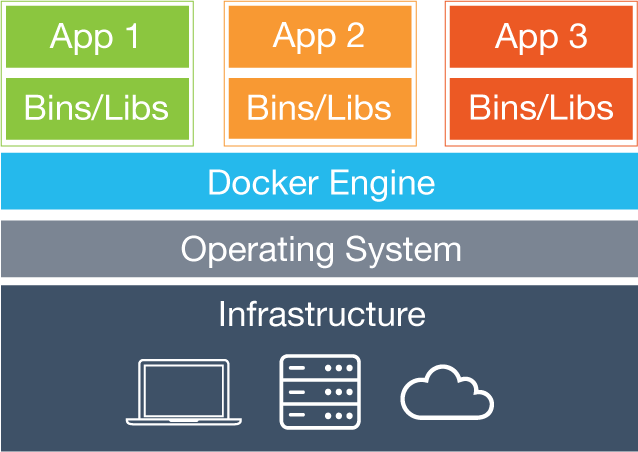
\includegraphics[scale=0.4]{5-patterns/images/what-is-vm-diagram.png}
% \paperwidth
\begin{center}
  \makebox[\textwidth]{
	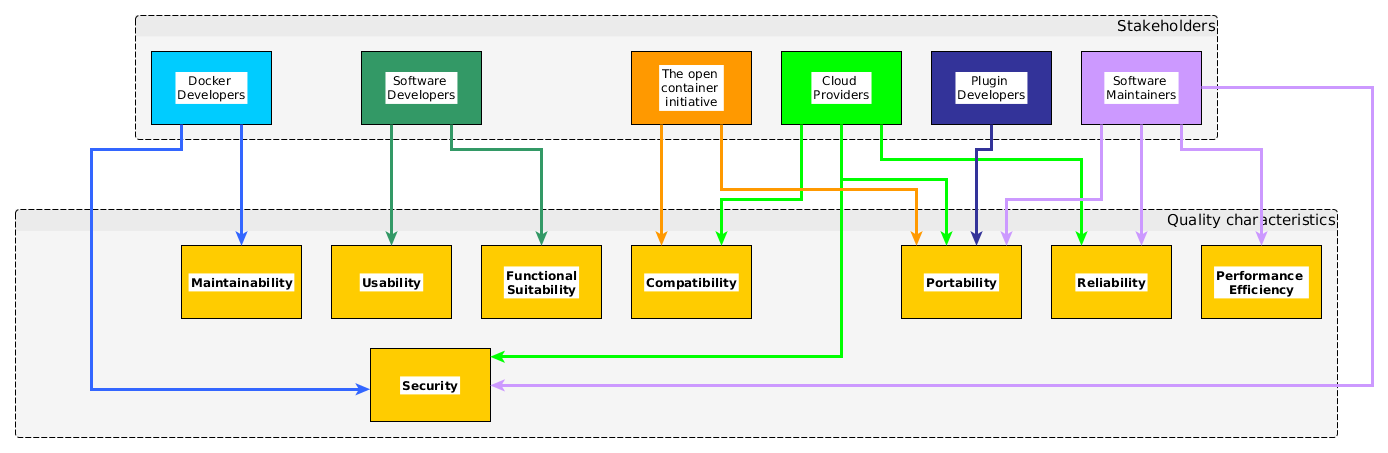
\includegraphics[width=0.9\paperwidth]{3-stakeholders/images/StakeholderQuality.png}
	}
%  \includegraphics[width=\paperwidth]{...}}
\end{center}
\caption{Stakeholders and the quality attributes they are concerned about}
\label{fig:stakeholders-quality}
\end{figure}



%
%\begin{table}[H] \centering
%	\caption{Matrix of stakeholders concern.}
%	\label{table:stakeholder_concern}
%	\begin{tabular}{@{} cl*{10}c @{}}
%		&  & \multicolumn{8}{c}{
%		\textbf{Concerns}} \\[2ex]
%		& \textbf{Stakeholder} 
%			& 
%			& \rot{Functional suitability}
%			& \rot{Performance efficiency}
%			& \rot{Compatibility}
%			& \rot{Usability}
%			& \rot{Reliability}
%			& \rot{Security}
%			& \rot{Maintainability}
%			& \rot{Portability}			
%			\\
%		\midrule
%								%ada	co-ex	impl	maint	perfor	port	relia	usa	
%& Software developer 	& &		&		&		&		&		&		&		X&		X 		\\
%& Software main 		& &		&		&		&		&		X&		X&		X&				\\				
%& Cloud providers 		& &		&		X&		X&		&		&		&		X&				\\			
%& The open container 
%initiative 				& &		&		&		&		&		&		X&		&				\\	
%& Docker developers 
%						& &		&		&		&		X&		&		&		&				\\				
%& Plugin developers 
%						& &		X&		&		&		&		&		&		&				\\				
%\midrule
%& Total					& &		1&	   1&	    1& 		1& 		1&		2&		3&		1		\\
%\midrule
%	\end{tabular}
%\end{table}

%!TEX root = ../report.tex

\section{Negative Stakeholders}
\label{sec:negativestakeholders}

% !TEX root = ../report.tex

\section{Key Drivers}
\label{sec:keydrivers}


Docker has the following key drivers
\begin{itemize}
	\item \req{kd}-- Portability
	\item \req{kd}-- Reliability
	\item \req{kd}-- Security
%	\item \req{kd}-- Compatibility
	%\item \req{kd}-- Maintainability
\end{itemize}
%
\subsection{Portability}
%
%Degree of effectiveness and efficiency with which a system, product or component can be transferred from one hardware, software or other operational or usage environment to another. This characteristic is composed of the following subcharacteristics:
%
%Adaptability. Degree to which a product or system can effectively and efficiently be adapted for different or evolving hardware, software or other operational or usage environments.
%Installability. Degree of effectiveness and efficiency with which a product or system can be successfully installed and/or uninstalled in a specified environment.
%Replaceability. Degree to which a product can replace another specified software product for the same purpose in the same environment.

%https://www.docker.com/
%Achieve agility and control for Development and IT Operations teams to build, ship, and run any app, anywhere

%https://github.com/docker/docker
% and are designed from the ground up with an application-centric design.”
%https://docs.docker.com/engine/installation/
Looking at Figure~\ref{fig:stakeholders-quality}, which visualizes the quality concerns of the stakholders, it is apparent that portability is the quality that is most desired among the stakeholders. One of the main features, if not the main feature of docker, is to provide ``agility and control for Development and IT Operations teams to build, ship, and run any app, anywhere'' \cite{dockermain}.\\
Docker want's the containers running the applications to be ``hardware-agnostic'' and ``platform-agnostic'' \cite{dockerrepo}, meaning that docker containers do not know anything about the hardware, nor the platform it is run on, thus making it very portable. This allows developers to focus on the actual application, without having to worry about the underlying hardware or platform. The applications the developers create could then be run everywhere where docker is supported.\\
To provide this quality attribute, Docker is also focused on increasing the performance. By making the docker containers small, yet having a high performance, the containers become usable by a wide variety of systems and are able to replace the need to use any virtual machines that would otherwise be used to achieve this level of portability. \cite{dockerrepo}\\
To increase the portability even more, the docker hub makes it very easy for docker containers to be shared and used on other machines.

\subsection{Reliability}
The main function of a docker container is to run a certain application. However, a system usually needs to run a set of different applications and should not be the case that running these applications in docker compromises the system's reliability.\\
Dependencies often lead to problems \cite{dockerrepo}, decreasing the reliability of software. The Docker files are text files containing a small set of instructions that will run an application. This means that the instructions needed to run an application are conveniently located in a single place, the docker files. This  allows viewing and the dependencies of all the different applications and making them easily maintainable.\\
Docker increases the reliability of the applications it runs, by increasing the testability of the containers and applications.\\
To make sure docker itself stays reliable, docker provides a test framework and test functions that thoroughly test docker.\\
% https://docs.docker.com/opensource/project/test-and-docs/
%
%makes systems and applications very maintainable.\\
%Dependencies of applications are centralized and easily manageable.\\
%Docker files are small text files, making it very share able. Instead of having to share an image of a VM, the docker file can be used to reuse an application or system anywhere.\\

%An application that is run on docker should not run slower and respond slower then if the application is not run in docker.\ign(natively) Database systems need to respond fast or anything that uses the database responds slow as well.\\
%The goal of a docker container is to run a certain application. However, a system usually needs to run a set of different applications and should not be the case that running these applications in docker compromises the system's resources.\\

\subsection{Compatibility}
The main goal of the docker project is to ``Build,Ship, and Run Any App, Anywhere'' \cite{dockermain}. To accomplish this, the docker containers need to be able to run on many different kinds of systems and platforms.\\
Docker containers behave like a virtual machine and can easily be configured to communicate with each other.\\
Docker also allows running the same application on multiple platforms. This allows the underlying operating system of an application to be changed, without compromising the system as a whole.


%\section{Stakeholders}
%\section{Negative Stakeholders}
%\section{Key Drivers}


%!TEX root = ../report.tex

\clearpage
\chapter{Software architecture}
\label{ch:softwarearch}
This section discusses the architecture of Docker.  Two views from the 4+1
Architectural View Model will be presented : the logical and the process view.

% !TEX root = ../report.tex

\section{Logical View}
\label{sec:viewlogical}

% Logical view : The logical view is concerned with the functionality that the system provides to end-users. UML Diagrams used to represent the logical view include Class diagram, Communication diagram, Sequence diagram.

Docker is made using the the go language created by Google. Docker is an application categorized as ``Operating-system-level virtualization''. It consists of:
\begin{itemize}
\item 2979205 lines of go code (allmost 3 million).
\item 1782 '.go' files
\item 267 different packages
\end{itemize}

If the main ``/docker'' package is build, the dependencies can be visualized using a  visualization tool. When restricting the depth to be 1, it produces the image below, Figure \ref{fig:dockerdep1}. The green node is the "main" node for which the dependencies are shown.

\begin{figure}[H]
\caption{A high-level overview of the Docker architecture.}
\centering
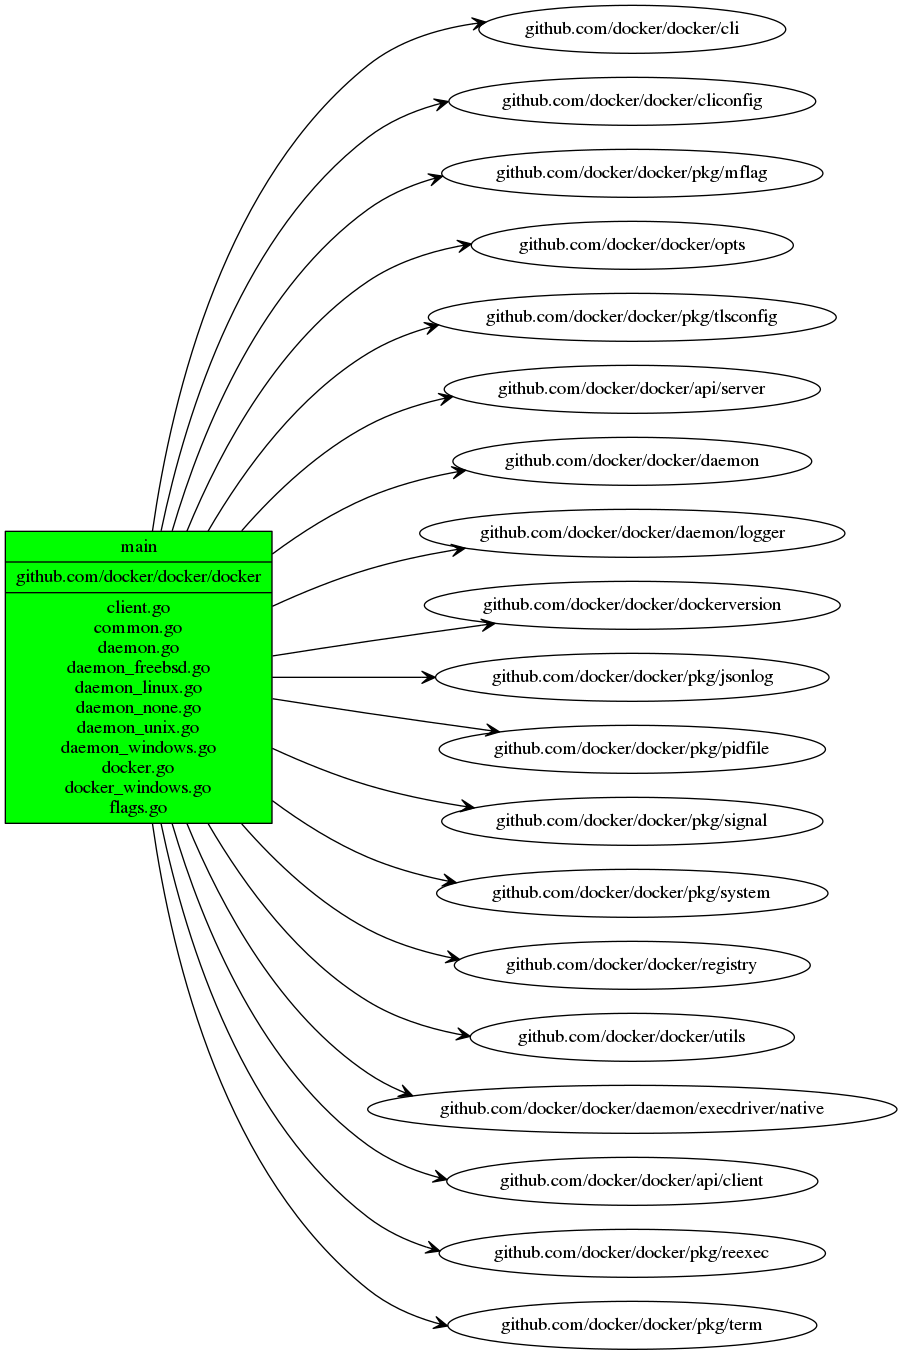
\includegraphics[width=\linewidth, height=15cm]{images/dependencyGraphs/goviz/govizgreendocker1.png}
\label{fig:dockerdep1}
\end{figure}

Looking at the official documentation, their image (Figure \ref{fig:dockerarchipic}) shows to be largely similar.\\

\begin{figure}[H]
\caption{A high-level overview of the Docker architecture. Source: \cite{dockerarchi}.}
\centering
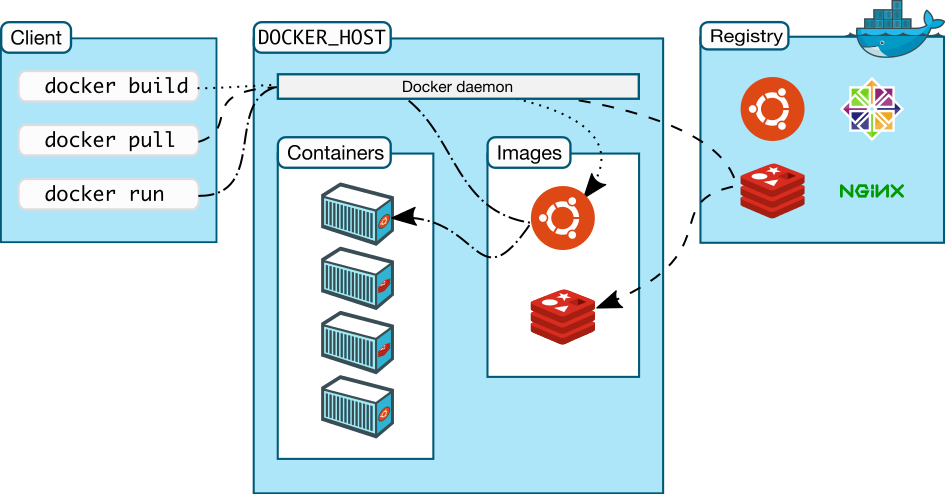
\includegraphics[scale=0.4]{4-softwarearch/images/architecture.png}
\label{fig:dockerarchipic}
\end{figure}
Docker uses a client-server architecture. The client (a command-line tool) acts as the primary user interface and talks to the Docker daemon. The daemon is a background process which dfig:dockerdep1oes all the heavy lifting, e.g. the building and running of the containers.


%TODO Research about the importance of the packages will be added still...
The most important part of docker will be discussed in the following sections below.

\subsection{Client}
The client is a small binary and acts as the primary user interface to Docker. The user enters command into the client and the client forwards these commands to the Docker daemon, which executes commands.
The Docker client is capable of connecting to daemons running on the local machine, as well as connecting to daemons running on remote machines over the internet.

\subsection{Server / Daemon}
The Docker daemon is a process running on the host machine (as can be seen in Figure~\ref{fig:dockerarchipic}). This process is started when the host machine starts and runs in the background. It exposes a REST interface and listens for requests coming from clients on the same or remote hosts.

\subsubsection{Images}
Docker images can be interpreted as a read-only template from which Docker containers are
started. A Docker image consists of a stack of layers which are bonded by union
file systems. These layers support reusability and sharing.

Docker images can be build from text files (`Dockerfiles'), which contain instructions like installing software and copying files.

\subsubsection{Containers}
% running usin libcontainer from the open specification
Docker containers are based on Docker images. This image acts as a read-only
layers. Then, Docker container adds a thin writable layer on top of it to
perform operations. Docker containers basically consist of the files of the operating system,
user-added files, application, and some information. Multiple containers may run
based on a same image. In this case, Docker will not create separate copies for
each containers. Instead, they will share same image with their own writable
thin layer.

To run Docker containers, Docker uses the \verb|libcontainer| library, which is part of the Open Container Initiative.

\subsection{Registry}
A Docker registry is a place where Docker images can be stored and retrieved. The Docker daemon
fetches desired Docker images from this repository. This registry may be a
public or a private one, such as one behind firewall. Docker
Hub\footnote{\url{https://hub.docker.com/}} is one example of a docker registry
hosted by Docker. A registry provides an easy way to distribute images between different hosts.


% % !TEX root = ../report.tex

\section{Development View}
\label{sec:viewdevelopment}

\subsection{Components}
% component diagram
%\newcommand{\main4ImgPath}{4-softwarearch/images/dependency/horizonDotWithS/}

\begin{figure}[H]
\centering
%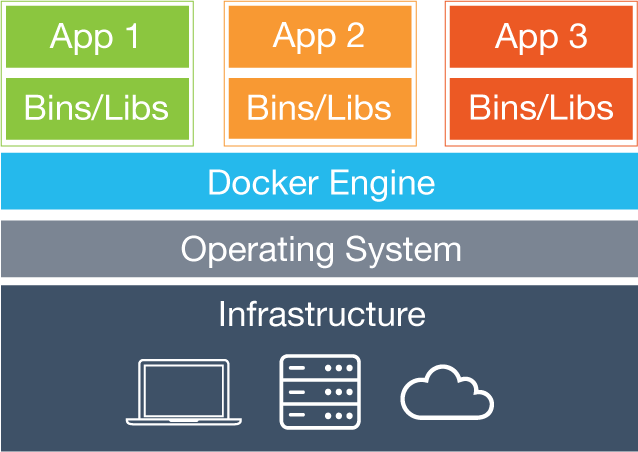
\includegraphics[scale=0.4]{5-patterns/images/what-is-vm-diagram.png}
% \paperwidth
\begin{center}
  \makebox[\textwidth]{
	\includegraphics[width=0.9\paperwidth]{4-softwarearch/images/dependency/horizonDotWithS/docker/dot.png}
	}
%  \includegraphics[width=\paperwidth]{...}}
\end{center}
\caption{Dependency graph docker}
\label{fig:dependency}
\end{figure}

\begin{figure}[H]
\centering
%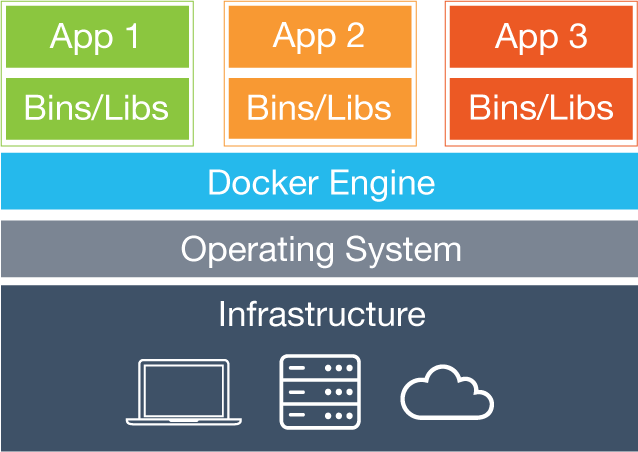
\includegraphics[scale=0.4]{5-patterns/images/what-is-vm-diagram.png}
% \paperwidth
\begin{center}
  \makebox[\textwidth]{
	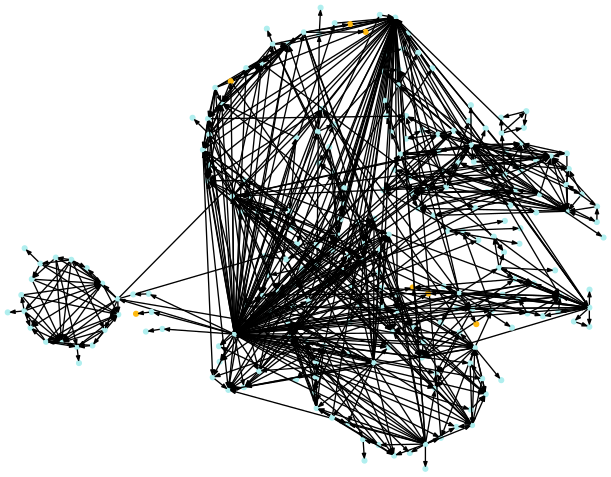
\includegraphics[width=0.9\paperwidth]{4-softwarearch/images/dependency/horizonDotWithS/daemon/circoPoint.png}
	}
%  \includegraphics[width=\paperwidth]{...}}
\end{center}
\caption{Dependency graph daemon circular}
\label{fig:dependency}
\end{figure}

\begin{figure}[H]
\centering
%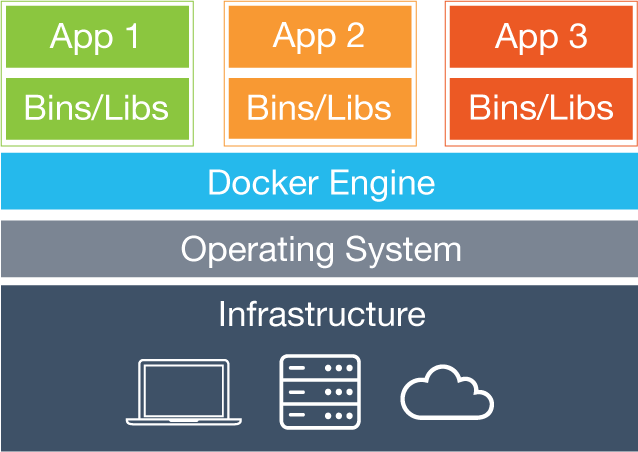
\includegraphics[scale=0.4]{5-patterns/images/what-is-vm-diagram.png}
% \paperwidth
\begin{center}
  \makebox[\textwidth]{
	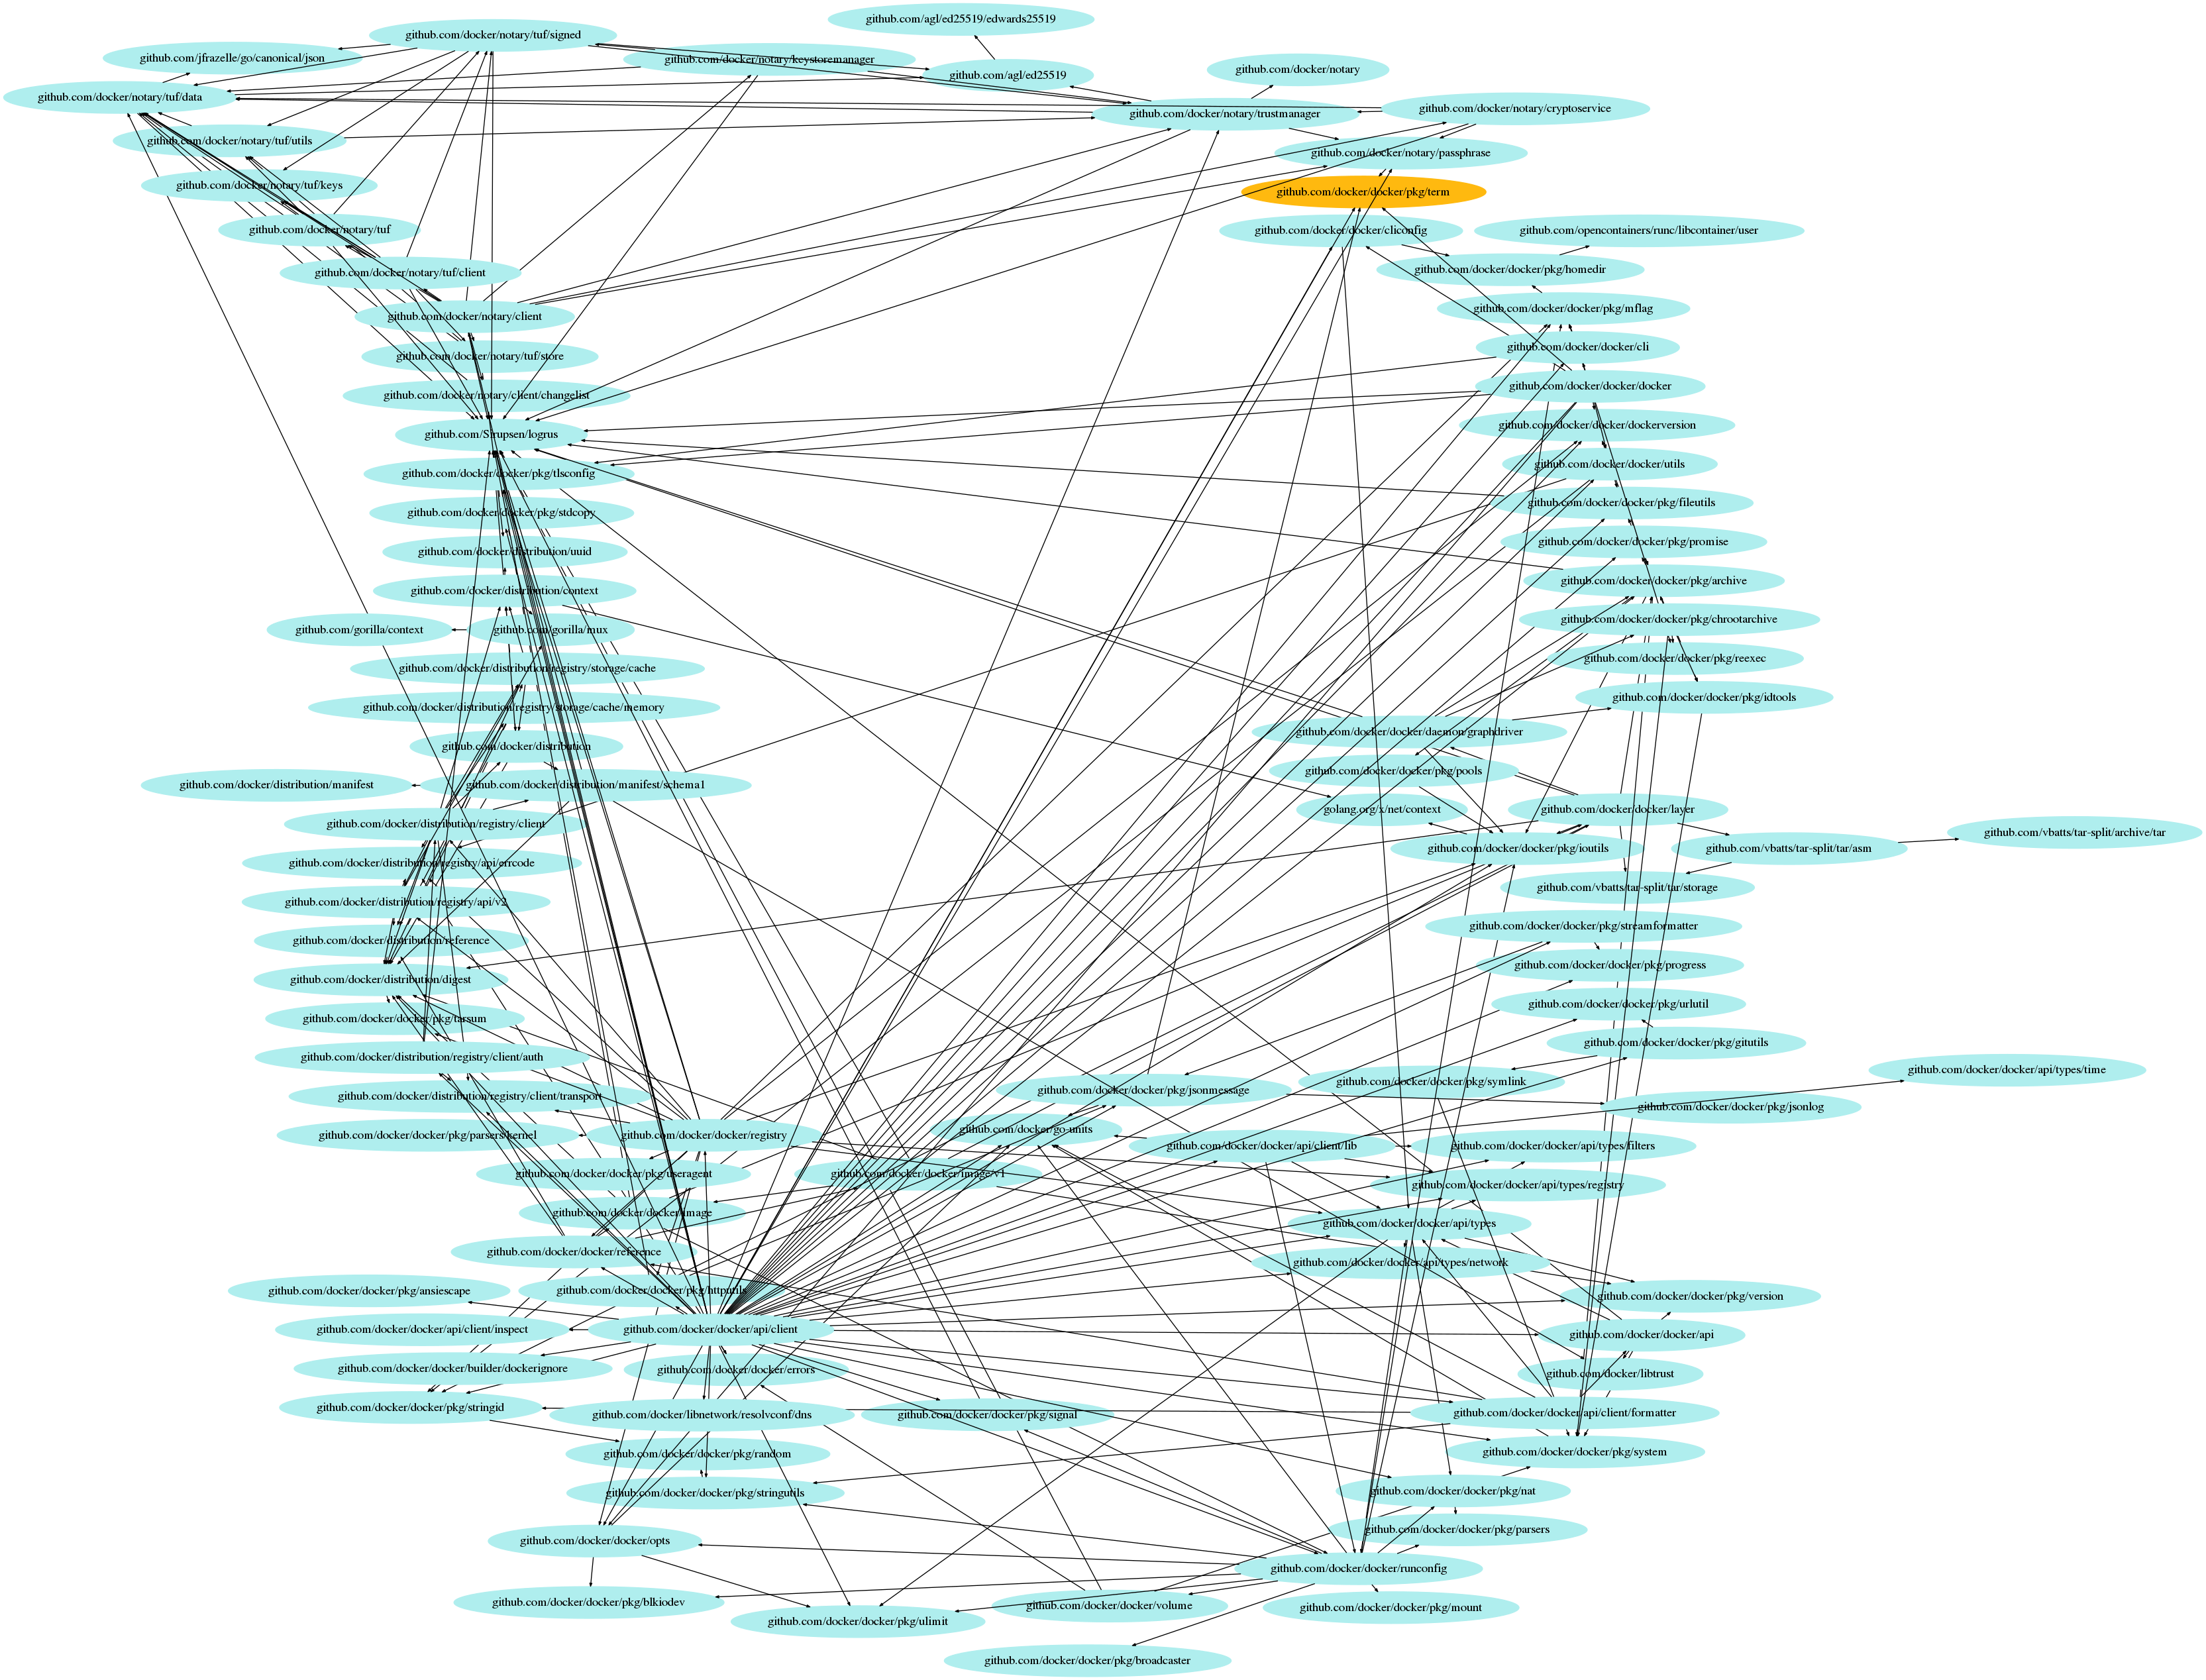
\includegraphics[width=0.9\paperwidth]{4-softwarearch/images/dependency/horizonDotWithS/docker/circo.png}
	}
%  \includegraphics[width=\paperwidth]{...}}
\end{center}
\caption{Dependency graph docker circular}
\label{fig:dependency}
\end{figure}



\begin{figure}[H]
\centering
%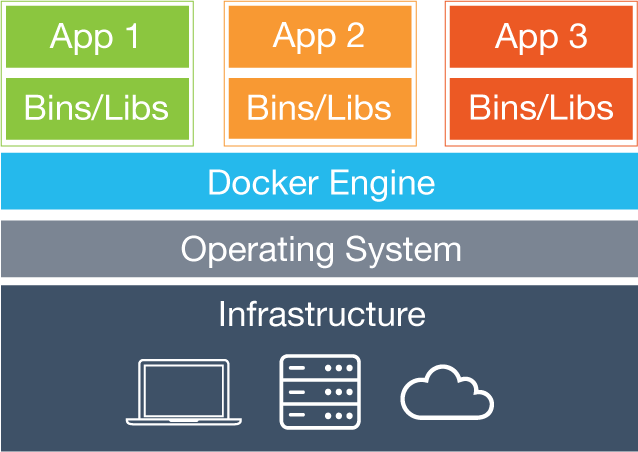
\includegraphics[scale=0.4]{5-patterns/images/what-is-vm-diagram.png}
% \paperwidth
\begin{center}
  \makebox[\textwidth]{
	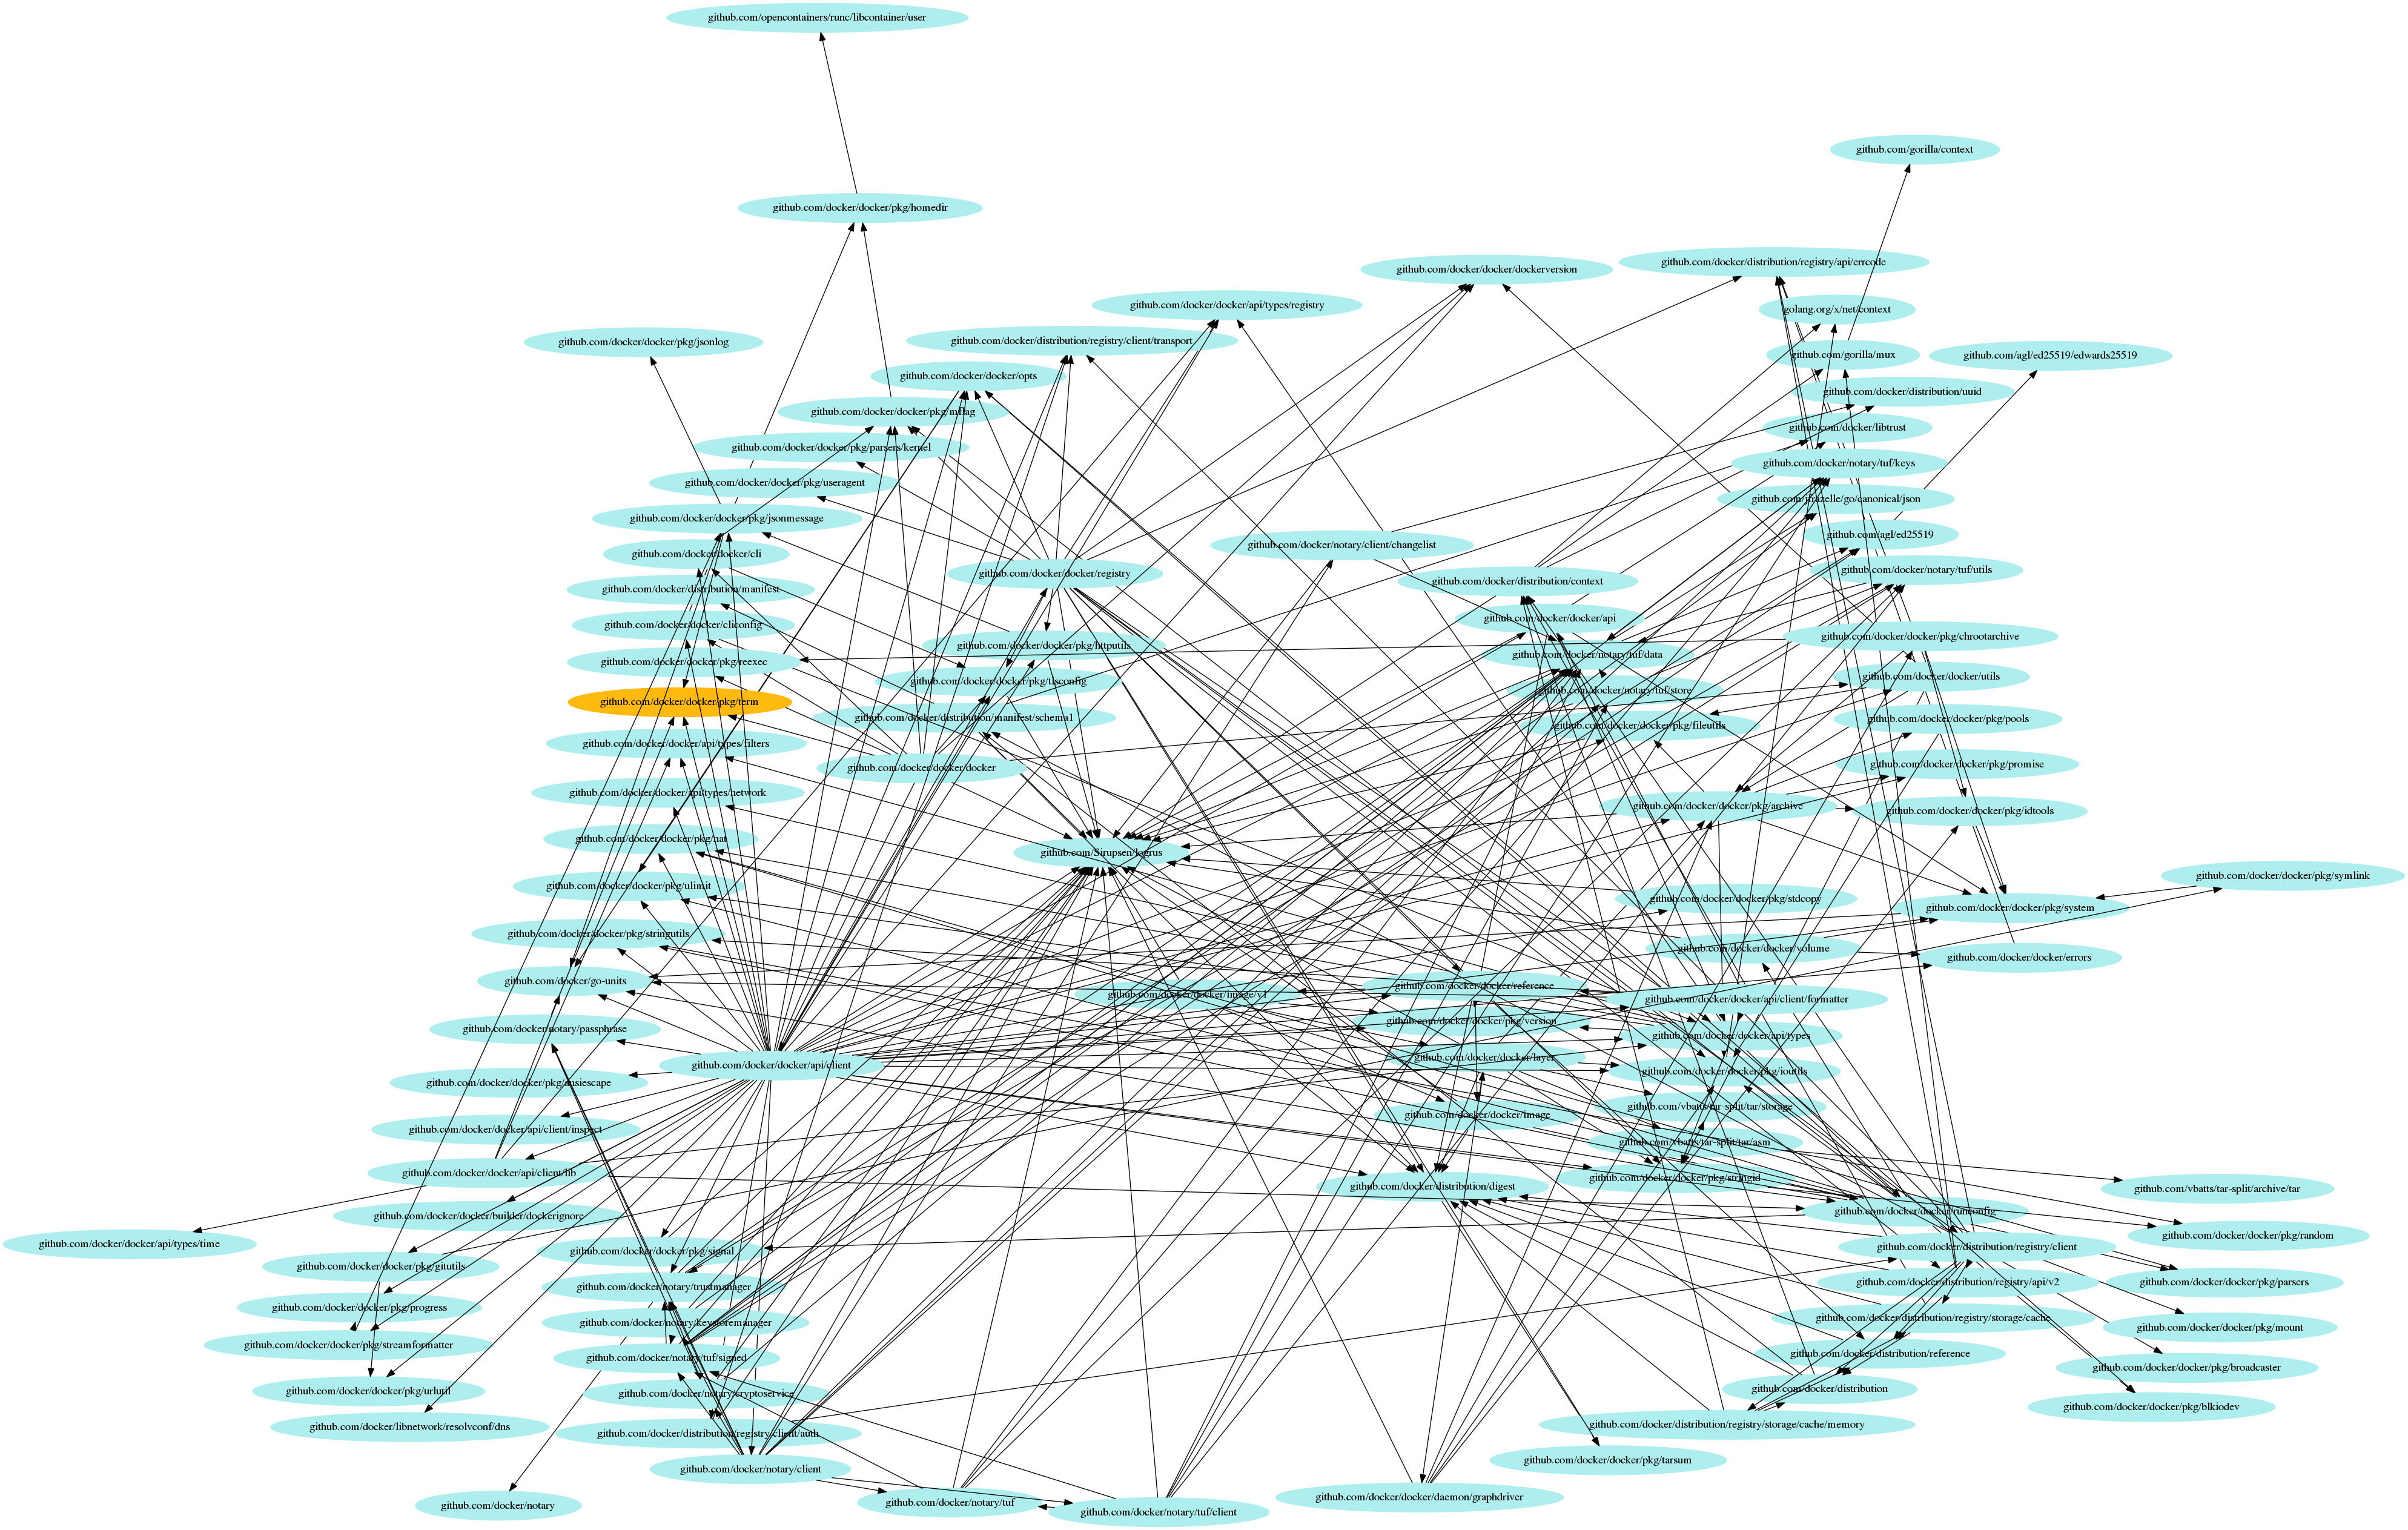
\includegraphics[width=0.9\paperwidth]{4-softwarearch/images/dependency/horizonDotWithS/docker/twopi.png}
	}
%  \includegraphics[width=\paperwidth]{...}}
\end{center}
\caption{Dependency graph docker}
\label{fig:dependency}
\end{figure}

\begin{figure}[H]
\centering
%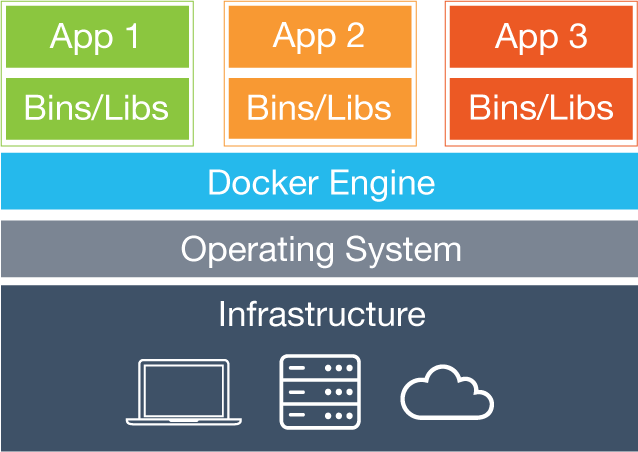
\includegraphics[scale=0.4]{5-patterns/images/what-is-vm-diagram.png}
% \paperwidth
\begin{center}
  \makebox[\textwidth]{
	\includegraphics[width=0.9\paperwidth]{4-softwarearch/images/dependency/horizonDotWithS/layer/dot.png}
	}
%  \includegraphics[width=\paperwidth]{...}}
\end{center}
\caption{Dependency graph layers}
\label{fig:dependency}
\end{figure}


% !TEX root = ../report.tex

\section{Process View}
\label{sec:viewprocess}
This section discusses the system processes, how they communicate and the runtime behaviour of the system.

\subsection{Plugins}
Docker supports extending its capabilities using third-party plugins. At the moment of writing, Docker allows extending the functionality of the volumes and network subsystems, which are responsible for storing files outside containers and inter-container communication over the network respectively. This will be extended in the future\cite{dockerplugindocs}.

A plugin runs in its own separate process and communicates with the Docker daemon using the REST API. In order for the Docker daemon to know about the plugins existence, a file has to be placed in a pre-defined directory. %todo explain exactly (sock file, etc file, json file ...)
In Figure~\ref{fig:activity_plugin} the process of using a plugin can be seen.
\begin{figure}[H]
\caption{An activity diagram showing the process of using a plugin (simplified)}
\centering
\includegraphics[scale=0.5]{4-softwarearch/images/plugins_activity.png}
\label{fig:activity_plugin}
\end{figure}

A user indicates that he/she wants to use a plugin by passing a command-line parameter to the Docker client when starting a container. If this parameter is present, then the daemon will start looking for the plugin in the plugin directory. If the plugin is not found, it returns an error to the user. 
When the plugin is found, the daemon will send a handshake to the plugin using a UNIX socket and the plugin will reply with a list of subsystems it implements. 
The Docker daemon will then use the \pattern{Proxy} pattern to forward calls to this subsystem to the plugin process.


%just two random views, because the example used them
%\section{Logical View}
%\section{Process View}


% !TEX root = ../report.tex

\clearpage
\chapter{Pattern Documentation}
\label{ch:patterns}
This chapter describes the patterns used in Docker identified by us. We documented the patterns as described by Harrison et al.\cite{usingpatternscapture}, with added information about where the pattern was found (traceability).

\section{Client-Server}

% see https://docs.docker.com/engine/introduction/understanding-docker/

\begin{description}
\item [Traceability]~\\
The Client-Server pattern can be deducted from the online documentation\cite{dockerarchi}.

The Client-Server pattern can be deducted from the `What is Docker’s architecture?' section of the online documentation\cite{dockerarchi}.

\item [Source]~\\
Architectural patterns revisited -- a pattern language, P. 29 \cite{avgeriou2005architectural}

\item [Issue]~\\
It should be possible for Docker containers to be controlled remotely and a single interface should be able to control containers on multiple hosts (e.g. in the cloud).

Additionally, certain operating systems lack the underlying technologies necessary for running containers. For those OSes, it should be possible to call remote daemons running on operating systems which are supported. % /WindowsBashing

\item [Solution]~\\
Docker uses a \pattern{Client-Server} architecture. The client, a binary supplying a command-line interface, act as the primary interface for the user. The user enters commands into this client, which are then send to a server: the Docker daemon. 


\item [Assumptions/Constraints]~
\begin{itemize}
\item The versions of the client binary and the server binary should match. Different versions can cause problems.
\item All the services offered by the daemon have to be made available to the client using a REST interface.
\end{itemize}
~\\[-1.7cm]
\item [Rationale] ~\\
The daemon is a background process, which supplies the requested services to the client. The daemon exposes a REST interface.

For Docker, the client can be configured to connect to other daemon processes than the one running on the local machine. It can be configured to connect to remote Docker daemons as well, allowing the user to issue commands to daemons running remotely.

%todo move above to architecture chapter 

By separating the client and server it is possible to use the same client to issue commands to different daemons, running on different hosts.
It is also possible to use the client on operating systems that do not support running containers.

\item [Implications]~\\
The use of the \pattern{Client-Server} pattern results in two different executable binaries: a daemon and a client. 

The use of the \pattern{Client-Server} pattern increases the interoperability, since the client can send commands to daemons running on remote machines and the local machine.

Additionally, the portability is increased, since the client can run on Operating Systems that cannot run containers themselves.


\item [Related Patterns]~\\


\end{description}

\clearpage
\section{Layers}
% see https://www.docker.com/sites/default/files/what-is-vm-diagram.png

% \begin{figure}[H]
% \centering
% 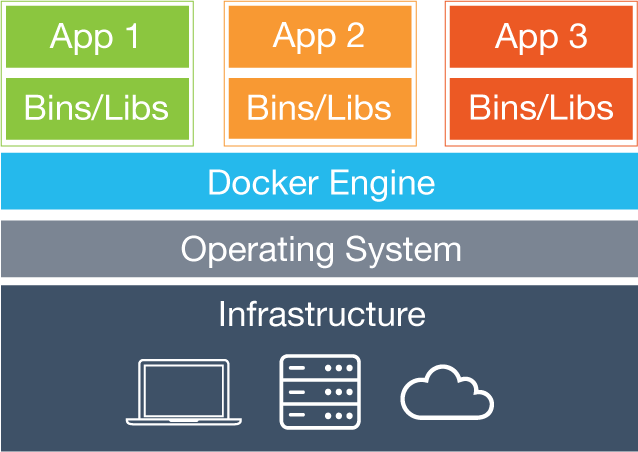
\includegraphics[scale=0.4]{5-patterns/images/what-is-vm-diagram.png}
% \caption{A layered overview of the Docker. Source \cite{whatisdocker}}
% \label{fig:layers-pattern}
% \end{figure}

\begin{description}
\item [Traceability]~\\
Layers is mentioned in the Docker architecture in the online documentation,
specifically in the explanation of Docker images\cite{dockerarchi}. \\
Furthermore, the user guide of Docker also elaborates on layers in the Docker images\cite{dockerimage}.

\item [Source]~\\
Architectural patterns revisited -- a pattern language, P. 29
\cite{avgeriou2005architectural}

\item [Issue]~\\
Docker emphasizes on developing containerization with almost no overhead. Running
multiple instances of Docker containers with the same image may end up in high
overhead. A sharing and reuse mechanism must be implemented to prevent overhead
and to save more space/resources.

\item [Assumptions/Constraints]~\\
An application running in a Docker container must have a CLI\footnote{Command Line
Interface} (bash), as Docker images are based on a Linux distribution.
%Wouter: not so sure about that, I saw a presentation once of somebody using volume mounts to have a program with GUI run in a Docker container

\item [Solution]~\\
Each Docker image consists of a stack of layers, which is read-only. The first
layer in the stack is a base image from a Linux distribution. Docker also
implements copy-on-write strategy. In this strategy, system processes that need
the same data share the same instance of data rather than having their own. A
copy will be made when a specific system process makes a change to the data (copy-on-write).

\item [Rationale] ~\\
Layers are very good in terms of sharing and reusability. In this way, overhead
can be avoided by sharing resources. A new image that uses same stack of layers
may reuse the layers rather than making a separate copy. This may result in
smaller sizes of Docker images.

\item [Implications]~\\
A Docker container will use Docker image as the base of it. This will remain as
read-only layers. Then, a Docker container will create another thin writable
layer on top of the image. Multiple containers that run based on the same Docker
image will not make their own copy of the image to prevent duplication.

This will end up in more efficient memory allocation (better performance efficiency).

\item [Related Patterns]~
\begin{itemize}
	\item Client-server
	\item Shared repository
\end{itemize}
\end{description}

% \clearpage


\section{Shared repository}
%\textit{Can we consider the docker registry a shared repository?}
% Schemas
%http://fr.slideshare.net/Docker/https-dldropboxusercontentcomu20637798docker-meetup-freiburg
% http://blog.octo.com/en/docker-registry-first-steps/   http://fr.slideshare.net/egorpushkin/docker-demo   
% Because of Pull/¨Push can we talk about Pattern publish suscribe ?   Asynhcronous Queuing ?

The docker registry is considered as a Shared Repository. \\
Two alternatives exist:DockerHub and Docker Trusted Registry. \\

Docker has a feature wich can be configured : the Notification Sytem which makes the Shared Repository an active Repository.
\textit{https://docs.docker.com/registry/notifications/}

\begin{description}
\item[Traceability]~\\
The Shared Repository pattern can be deducted from the online documentation : \textit{https://docs.docker.com/registry/} ``The Registry is a stateless, highly scalable server side application that \textbf{stores} and lets you \textbf{distribute} Docker images. A registry is a storage and content delivery system.''

% File store.go , registry.go

\item[Source]~\\
%\EAA, P.322 \cite{eaa}\\
Architectural Pattern Revisited - A Pattern Language, P.13 \cite{avgeriou2005architectural}

\item[Issue]~\\
Docker provided a way for the user to conrol the storage and distribution of images. \\
The user wants to be alerted of new events happening in the registry through notifications. % Develop ?

%\item[Assumptions/ Contrainst]~\\

\item[Solution]~\\ %how does it work ?
Users interact with a registry by using docker push and pull commands.

\item[Rationale]~\\ % in which way this pattern helps Docker? What is the goal ? KD
 After the integration of the Shared Repository Pattern each has one central repository containing their images and they can it access using a loggin. \\

\item [Related Patterns]~\\
Event-driven Messaging

\item [Related Quality Attributes/Key drivers]~\\
Reusability, Changeability, Maintainability, Integrability

 \begin{figure}[H]
 \centering
 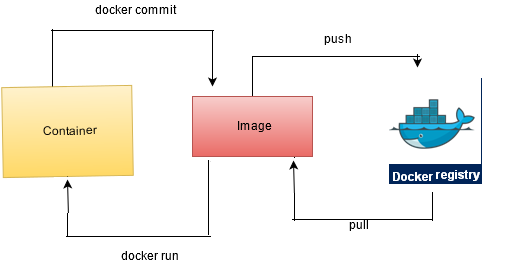
\includegraphics[scale=0.7]{images/Dockerrep.png}
 \caption{Docker Regitry}
 \label{fig:docker-registry}
 \end{figure}

\end{description}

\section{Event-Driven Messaging}

\begin{description}

\item[Traceability]~\\
The notification mechanism of the Docker Registry uses the Even-Driven Messaging Pattern.

\item[Source]~\\
http://soapatterns.org/designpatterns/eventdrivenmessaging

\item[Issue]~\\ The user wants to be alerted about certain events occuring in his registry.
The notification system needs a mechanism in order to send the events to the user.

\item[Assumptions/Contrainst]~\\ This pattern is used at a lower level in the Docker Registry/Active Repository Pattern.

%\item[Solution]~\\

\item[Rationale]~\\ 

\quote {"Notifications are sent to endpoints via HTTP requests. Each configured endpoint has isolated queues, retry configuration and http targets within each instance of a registry. When an action happens within the registry, it is converted into an event which is dropped into an inmemory queue. When the event reaches the end of the queue, an http request is made to the endpoint until the request succeeds. The events are sent serially to each endpoint but order is not guaranteed."}

\item [Related Patterns]~\\
Active Repository Pattern

%\item [Related Quality Attributes/Key drivers]~\\

\end{description}

\begin{figure}[H]
\centering
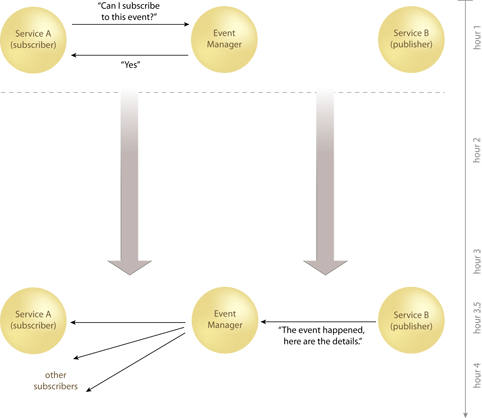
\includegraphics[scale=2]{images/EDM.png}
\caption{Event-Driven Messaging}
\label{fig:event-driven}
\end{figure}

\section{Direct Authentication}
%Brokered Authentication


\begin{description}

\item[Traceability]~\\
The Direct Authentication pattern can be deducted from the source code through the "auth.go" file from the Docker Github Repository. \\
The notification mechanism of the Docker Registry uses this pattern.
\quote{Since securing access to your hosted images is paramount, the Registry natively supports TLS and basic authentication.}

\item[Source]~\\
\textit{https://msdn.microsoft.com/en-us/library/ff647715.aspx} \\
%http://soapatterns.org/design_patterns/direct_authentication
%https://docs.docker.com/registry/spec/auth/token/


\item[Issue]~\\ The Docker Registry needs an authentication system in order to ensure security for the user through a login.

%\item[Assumptions/Contrainst]~\\ 

\item[Solution]~\\ By using the Direct Authentication the access to the Docker Registry is controlled for each user.

\item[Rationale]~\\ 

\item [Related Patterns]~\\
Shared/Active Repository Pattern

\item [Related Quality Attributes/Key drivers]~\\
Security

\end{description}

\section{Plugin}
\label{sec:pattern-plugin}
%TODO image
\begin{description}

\item [Traceability]~\\
The existence of Docker Plugins becomes apparent from it's documentation at \cite{dockerplugindocs}.

Additionally, the directories \verb|docker/pkg/plugins/| \footnote{\url{https://github.com/docker/docker/tree/master/pkg/plugins}} and \verb|  docker/daemon/graphdriver/plugin.go| \footnote{\url{https://github.com/docker/docker/blob/master/daemon/graphdriver/plugin.go}} (among others) in the project's repository contain the code for discovering plugins and the interfaces the plugins should implement.

\item [Source]~\\
Patterns of Enterprise Application Architecture, P. 499 \cite{eaa}

\item [Issue]~\\
The users of Docker want to have customization, by extending Docker with third party custom-built tools. This customization means that third parties should be able to write plugins that extend Docker's core functionality.\cite{dockerpluginblog}

The implementation of such plugins is only available at runtime.

\item [Assumptions/Constraints]~
\begin{itemize}
\item Plugins can only extends the functionality of the components of Docker, that have an interface that plugins can implement.
\end{itemize}


\item [Solution]~\\
Docker uses the Plugin pattern to link the implementation of the interfaces of several extendable components with third-party implementation at runtime.

\item [Rationale] ~\\ % https://docs.docker.com/engine/extend/plugin_api/
Docker discovers plugins by looking for .sock, .spec or .json files in the plugin directories on the host system. These files describe how Docker can communicate with the plugins using the REST API (usually via a Unix socket).

The plugins themselves run as separate processes on the same host as the Docker daemon and implement an HTTP server listening for requests from the Docker daemon. After a user requires a plugin (this is indicated e.g. as a command-line parameter when starting a container using the Docker client) Docker uses the discovery algorithm (see also Section~\ref{sec:processplugins}). After that, Docker sends a handshake to the plugin and the plugin returns a list of which subsystems this plugin implements.


For these subsytems Docker will replace the default implementation by a Proxy, that forwards all calls over the REST interface to the plugin process.

\item [Implications]~\\
The use of the Plugins pattern means that the adaptability increases. 

\item [Related Patterns]~
\begin{itemize}
\item Proxy
\end{itemize}
\end{description}

\section{Proxy}
\begin{description}

\item [Traceability]~\\
The use of the \pattern{proxy} pattern becomes apparent from the source code in the repository on GitHub.
For example, the proxy for the Volumes plugin can be found in \verb|docker/daemon/graphdriver/proxy.go| \footnote{\url{https://github.com/docker/docker/blob/master/daemon/graphdriver/proxy.go}}.

\item [Source]~\\
Pattern-oriented Software Architecture - Volume 4, P.290 \cite{wiley4}

\item [Issue]~\\
The plugins are separate processes than the daemon and are only available at runtime. Therefore, it is impossible for the daemon process to access the services of the plugins directly.
% issue also for comms between client-server ??

\item [Assumptions/Constraints]~
\begin{itemize}
\item The plugins have to implement a server listening for requests from the daemon.
\end{itemize}

\item [Solution]~\\
Let the daemon only communicate with the plugins through a proxy. This proxy implements all the `housekeeping' functionality, like sending API requests and authentication. It has the same interface as the plugin. \\
Whenever a call is done from the daemon to the plugin, it goes via the proxy, which communicates this call using a REST API to the plugin process.

\item [Rationale] ~\\ 
Using the \pattern{proxy} pattern allows the daemon to communicate with the plugins, without requiring direct access to these plugins. \\
Also, because the subsystem component has the same interface as its proxy, the implementation of software using this component does not depend on whether the proxy is used or the original subsystem. 

\item [Implications]~\\
The use of the \pattern{proxy} pattern allows communication with the plugins, which increases the extendability. 
Because the communication with the process is not direct, there is some performance overhead.
%TODO: what about portability??

\item [Related Patterns]~
\begin{itemize}
\item Plugin
\end{itemize}

\end{description}



% !TEX root = ../report.tex

\clearpage
\chapter{Evaluation}
\label{ch:evaluation}
This chapter presents the evaluation of documented patterns and overall system
against the key drivers of the architecture which already presented in Chapter
\ref{ch:stakeholders}. PBAR\cite{pbar} method is used to carry out the
evaluation. Force Resolution Maps (FRM) are also utilized to present the result.

\begin{table}[H]
\centering
\caption{Force Resolution Maps definition.}
\label{tab:frm-table}
\begin{tabular}{cl}
\textbf{Value} & \textbf{Definition} \\ \toprule
            $-2$   & Big negative impact \\
            $-1$   & Small negative impact \\
            $0$    & Neutral \\
            $+1$   & Small positive impact \\
            $+2$   & High positive impact 
\end{tabular}
\end{table}

\section{Patterns}
\subsection{Client-Server}
\subsection{Layers}
\begin{figure}[H]
\centering
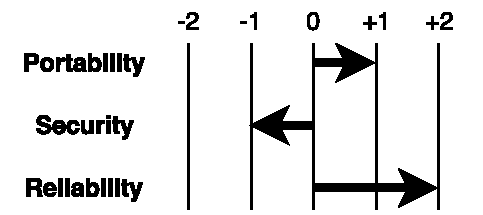
\includegraphics[scale=0.7]{6-evaluation/images/layers_frm.pdf}
\caption{Force Resolution Map for Layers pattern.}
\label{fig:layers-frm}
\end{figure}
This pattern gives positive implication to portability as clear separation of
containers, Docker daemon, Docker registry, and Docker client makes Docker
portable and loosely coupled. Utilizing Docker registry also promotes sharing
images, which make it easier to deploy an application without knowing what
platform running below it. Exposing TCP/IP connection, specifically REST,
contributes to negative effect on the security. It means that any unwanted
connections or attacks could possible exploit this hole. However, this weak
point is compensated by other patterns. Furthermore, Decoupling some components
means that the components below or above can be replicated in order to gain more
reliability as it has more availability. Thus, this patterns give positive
effect to the reliability. The summary of the Layers pattern evaluation is shown
in FRM in Figure \ref{fig:layers-frm}.

\subsection{Shared repository}
\subsection{Event-Driven Messaging}
\subsection{Direct Authentication/Brokered Authentication}
\subsection{Plugin}
\begin{figure}[H]
\centering
\includegraphics[scale=0.7]{6-evaluation/images/plugin_frm.png}
\caption{Force Resolution Map for Plugin pattern}
\label{fig:plugin-frm}
\end{figure}
The Plugin pattern greatly increases the portability, because it increases the adaptability by allowing third parties to develop extensions for Docker. 

It has a slight negative impact on the security, because there is communication between the daemon and plugin process which has to be secured. Additionally, the security of the plugins is not controlled by Docker, so defects in a plugins security can affect the security of the Docker daemon as well. 

There are no significant impacts on the reliability because of this pattern.

\subsection{Proxy}

\section{Overall system}

% !TEX root = ../report.tex

\clearpage
\chapter{Recommendations}
\label{ch:recommendations}
Table \ref{tab:qa-overview} shows the overview of the patterns and the implications on the key drivers. According to this table, the docker architecture is doing very well at increasing support for the main key driver: portability, while showing no particular effect for the other key drivers: security and reliability.\\
Docker is used a lot in the cloud to host certain services. Networking capabilities are this essential to Docker and directly effect the key drivers. It seams however, that certain aspects of Docker might negatively influence the an otherwise positive aspect of a pattern. This means that some patterns arent used in their full potential, thus giving the opportunity to increase key drivers.
Though Docker is doing very well at positively influencing their main key driver, there are some recommendations that might improve their key drivers. These recommendations are discussed in this chapter \\

\section{Networking}
Networking is done using a broker pattern, yet modifying the configuration of the networking seems to be very hard. This is because the networking is done by the docker daemon, only accessible using the client. So modification of the networking of docker has to be supported by the docker daemon and the docker client in order to work.\\
The functionality is there, however. So improving the networking functionality might be achieved by delegating the task of modifying the  configuration using already available services. The daemon is only required to provide the security by authenticating the request using the brokered authentication. The docker daemon could, for example, delegate docker client commands to ssh commands in the networking configuration of the container. \\

\section{Connectivity}
Docker containers are lacking capabilities to connect to each other. It is possible to let a docker container use an other docker container, but the functionality is very limited. For example, it does not seem possible to link the containers in a circular way.\\
Though the key drivers are not directly effected, interoperability is decreased. An application can still build and run everywhere, but only as stand-alone application.\\
This is something that the stakeholders would really like to have. In the architecture there is a layer pattern that clearly defines the functionality a layer should have. However, these layers do block the ability to communicate with an other docker container. Making the layers more accessible might improve the interoperability container capabilities. This will probably require modifications of the layers, redefining their functions. Doing so means modifications throughout the entire system, because all other patterns (broker, client-server, Plugin, publish-subscribe) need these layer definitions in order to function.

\section{security}
The security that is provided by the docker hub is not open source. Nautilus is the tool that is used to scan the images and this uses proprietary code.\\ 
Though it might secure the docker hub, docker registries that are not hosted by docker lack this security. This can negatively influence the security of docker greatly.\\
If docker were to use open-source security solutions, the overall security of docker would increase because then security would be easily available to the registries that are hosted on-premise.\\
Docker recently stated however that \q{But as of right now there are no plans to open source the scanning techniques}.

\section{Windows support}
Because the Docker daemon uses Linux-specific kernel features, you are unable to run Docker native in Windows. \\
Docker could try and create a layer that can communicate with windows as well. Doing so might be a lot of work though, but if they really want Docker application to be able to ``run everywhere'', they need to provide this functionality.


%!TEX root = ../report.tex

\clearpage
\chapter{Conclusion}
\label{ch:conclusion}
% \section{Pattern-Based Architecture Reviews}
% \section{IDAPO}

% %sounds like we're about to die...
% \section{Final Words}

This document have presented the architecture recovery of Docker by identifying
software patterns and performing an evaluation of the architecture based on the
identified patterns according to their impact on the Docker's quality
attributes. This is done by implementing PBAR and IDAPO method. IDAPO method is
used to identify the patterns within the Docker architecture, while PBAR is
utilized to perform the architecture review.

We firstly start by grasping some basic information about Docker. The findings
were presented in the System Context chapter, which consists of brief
explanation about Docker and its ecosystem, along with the communities
supporting and developing it. We then figured out the stakeholders behind Docker
project and their concerns. Based on our findings, the stakeholders can be
grouped in to six groups, those are Docker developers, Software developers that
utilize Docker in their project, the Open Container Initiative, cloud providers,
Docker plugin developers, and software maintainers. The summary of stakeholders
and their concerns can be seen in Figure \ref{fig:stakeholders-quality}. Based
on their concerns, the key-drivers can be extracted and those are
\textit{portability, security, and reliability}.

Even if software designers or developers may not be aware of certain software
patterns, the patterns may still be present \cite{idapo}. The IDAPO process is
used to identify existing patterns in a open source software. Patterns recovery
is very useful for quantifying the software project on a high-level approach. By
knowing the patterns inside a particular software project it is also easier to
measure or evaluate it by their impact to the software's key-drivers. The IDAPO
consists of 12 iterative steps that aim to achieve a robust pattern recovery
inside the OSS project. The mapping of IDAPO process and the chapters of this
document is described in chapter \ref{ch:introduction}.

A typical evaluation of an architecture requires a lot of effort and cost, for
example, ATAM method. PBAR provides a lightweight architecture review process
that can be used where traditional architecture review methods would not because
of their high cost. PBAR focuses the evaluation on issues of the system's' key-
drivers. It makes use of discovered patterns within the architecture to properly
document issues. PBAR consists of four main steps, which the third step, the
review meeting, is actually a repetitive steps.

One of the reason why Docker is selected to be the target of this Pattern-based
recovery and evaluation is of its popularity. The purpose this software is to
make the deployment of distributed application easier. As stated in the
documentation, Docker provides an integrated technology stacks, which enables
the development and IT operation teams to build, ship, and run distributed
applications anywhere without having to know the platform running below it.

Our investigation showed that there are seven layers exists in Docker, although
more patterns are likely to be there as well. The detailed documentations of
those pattern are written in chapter \ref{ch:patterns}. In this project, we also
implemented some insight that we achieved when working with the first project of
Software Pattern. Hopefully, the enhanced insights and experiences of this
second assignment would be beneficial for us in the future.


%!TEX root = ../report.tex
%\cleardoublepage
%\clearpage
%
%\appendix
%\appendixpage
%\addappheadtotoc

\begin{appendices}
			
	%\addcontentsline{toc}{part}{\appendixname}
				
	\renewcommand{\thechapter}{\Alph{chapter}}
	\renewcommand{\thesection}{\thechapter.\arabic{section}}
	\renewcommand{\thesubsection}{\thesection.\arabic{subsection}}
	\renewcommand{\thesubsubsection}{\thesubsection.\arabic{subsubsection}}

	% !TEX root = ../report.tex
\chapter{Time Tracking}
\label{App: Time Tracking}
% STRUCTURE:
%\begin{longtable}{p{0.2\textwidth} p{0.7\textwidth} p{0.1\textwidth}}
%	\textbf{Person} & \textbf{Task} & \textbf{Hours} \\ \toprule
%	Putra           &	&	\\ \midrule
%	Fakambi         &	&	\\ \midrule
%	Schaefers       & 	& 	\\ \midrule
%	Menninga        &	&	\\ \bottomrule
%\end{longtable}

\section*{Week 1}
\begin{longtable}{p{0.2\textwidth} p{0.7\textwidth} p{0.1\textwidth}}
	\textbf{Person} & \textbf{Task} & \textbf{Hours} \\ \toprule
	Putra           & Coaching session, researching about Docker, working on first draft of introduction 	& 3.5	\\ \midrule
	Fakambi         & Coaching session, Research about Docker, Work on the system context & 3.5	\\ \midrule
	Schaefers       & Coaching session, setting up initial layout and new git repository, defining key drivers, research. &  6.5 	\\ \midrule
	Menninga        & Coaching session, stakeholders and concerns & 4.0 \\ \bottomrule
\end{longtable}

\section*{Week 2}
\begin{longtable}{p{0.2\textwidth} p{0.7\textwidth} p{0.1\textwidth}}
	\textbf{Person} & \textbf{Task} & \textbf{Hours} \\ \toprule
	Putra           & Catching up after winter break, reading Docker docs, revising intro, and writing layers pattern documentation & 6	\\ \midrule
	Fakambi         & Coaching session, Meeting for discussing the patterns & 3 \\ \midrule
	Schaefers       & Creating scripts to find patterns, building and running docker, creating various dependency graphs, changing the key driver section, adding stakeholders and concern image & 8.5 \\ \midrule
	Menninga        & Searching patterns, improving stakeholders, client-server and plugin patterns. Improvements to System context. & 7.5 \\ \bottomrule
\end{longtable}

\section*{Week 3}
\begin{longtable}{p{0.2\textwidth} p{0.7\textwidth} p{0.1\textwidth}}
	\textbf{Person} & \textbf{Task} & \textbf{Hours} \\ \toprule
	Putra           & Coaching session, reading docker documentation and source code, revising intro and layers pattern, small changes in logical view and evaluation & 14.5	\\ \midrule
	Fakambi         & Coaching Session, small modifications System Context, Work on the Shared Repository, Event-Driven and Direct Authentication &	12\\ \midrule
	Joris 			& Researching and generating dependency graphs. Coaching session (via skype). Adding a software architecture begin. & 11 \\ \midrule
	Menninga        & Coaching session, improvements after feedback, process/logic view, client-server, plugin, proxy, changed key drivers & 15 \\ \bottomrule
\end{longtable}

\section*{Week 4}
\begin{longtable}{p{0.2\textwidth} p{0.7\textwidth} p{0.1\textwidth}}
	\textbf{Person} & \textbf{Task} & \textbf{Hours} \\ \toprule
	Putra           & Coaching session, meetings, group 3 review, working on feedback, rewrite and add illustration and evaluation for layers pattern, first draft of conclusion. & 	\\ \midrule
	Fakambi         & & \\ \midrule
	Joris 			& & \\ \midrule
	Menninga        & Coaching session, meetings, reviewing document other group, evaluation for patterns, improvements to patterns & 12 \\ \bottomrule
\end{longtable}
	
\end{appendices}

\bibliography{library}

\end{document}